\documentclass[11pt]{article}
\usepackage[a4paper,margin=27mm]{geometry}
\usepackage[T1]{fontenc}
\usepackage{lmodern,microtype,amsmath,amssymb,amsthm,mathtools,enumitem}
\usepackage{xcolor}
\usepackage{tikz}
\usepackage[colorlinks=true,linkcolor=blue,citecolor=blue,urlcolor=blue]{hyperref}
\hypersetup{pdftitle={Coherence, Dominance, and Generalized Loss},hypertexnames=false}
\newtheorem{theorem}{Theorem}[section]
\newtheorem{lemma}[theorem]{Lemma}
\newtheorem{proposition}[theorem]{Proposition}
\newtheorem{corollary}[theorem]{Corollary}
\theoremstyle{definition}
\newtheorem{example}[theorem]{Example}
\theoremstyle{remark}
\newtheorem{remark}[theorem]{Remark}
\newcommand{\R}{\mathbb R}
\newcommand{\N}{\mathbb N}
\newcommand{\M}{\mathcal M}
\newcommand{\C}{\mathcal C}
\newcommand{\U}{\mathcal U}
\newcommand{\PP}{\mathcal P}
\newcommand{\G}{\mathcal G}
\newcommand{\Lf}{\mathfrak L}
\newcommand{\one}{\mathbf 1}
\newcommand{\supp}{\operatorname{supp}}
\setlist{itemsep=1pt,topsep=3pt}

\title{Coherence, Dominance, and Generalized Loss}
\author{Jason Konek and Catrin Campbell-Moore}
\date{October 2026}

\begin{document}
\maketitle

\begin{abstract}
A dominance argument for coherence has two halves: every coherent model is undominated, and every incoherent model is dominated by a coherent model that is itself undominated. We study when such arguments succeed for arbitrary models, arbitrary sets of worlds and arbitrary rankings, which need not be numerical, complete or transitive. We separate three questions. First, what follows once every model is weakly dominated by an undominated coherent model? With one condition on ties, the undominated models are then exactly the undominated coherent ones; and if every coherent model is undominated under some ranking, the rationally permissible models are exactly the coherent ones. Second, which conditions, checkable without knowing the conclusion, ensure that such replacements exist? For rankings given by losses it suffices to assign to each prior an undominated coherent model that is a Bayes model for some prior supported within the support of the first, with losses that vary lower semicontinuously; for infinitely many worlds the assigned models must belong to one compact family, and an example shows that this cannot be dropped. Behind these results lie general theorems for arbitrary rankings, proved by the lemma of Knaster, Kuratowski and Mazurkiewicz on finite sets of worlds and compactness. Third, how can suitable rankings be constructed? A short proposition reduces this to the existence of improvements of a specific kind. Applications include probabilism on arbitrary domains under lower semicontinuity at each world, proper scores, conditional reports given events of probability zero, and a counterexample to a theorem of Joyce.
\end{abstract}

\section{Introduction}\label{sec:intro}

Many arguments for coherence share one shape. Models of some kind, such as credence functions, forecasts or sets of desirable gambles, are assessed by how well they perform in each possible world. The argument then shows two things: no coherent model is dominated, and every incoherent model is dominated by a coherent one that is not itself dominated. De Finetti's argument from sure loss has this shape~\cite{deFinetti}, and so do the accuracy-dominance arguments for probabilism~\cite{Joyce,Predd,SSK09,Pettigrew,Nielsen}. The complete class theorem of statistical decision theory~\cite{Wald} is a relative: it identifies the undominated decision rules with Bayes rules and their limits, among randomised rules.

This paper studies such arguments in a general setting. Models carry no structure, the set of worlds is arbitrary, and a model's performance at a world is assessed by a ranking: a binary relation at each world that need not be numerical, complete or transitive. The coherent models form a class fixed in advance. A family of rankings is given, each regarded as a reasonable way to assess performance at the task at hand. We ask when the undominated models of each ranking are exactly its undominated coherent models, and when every incoherent model is dominated by one of them. The paper is organised around three questions.

\emph{What follows once coherent undominated replacements exist?} Section~\ref{sec:conclusion} takes as given the \emph{dominance conclusion}: every evaluable model is weakly dominated by an undominated coherent model. Together with one condition, that a model tied at every world with an undominated coherent model is itself an undominated coherent model, this identifies the undominated models exactly. Applied across a family of rankings, and given that every coherent model is undominated under some ranking in the family, it shows that the rationally permissible models are exactly the coherent ones. Only one of these consequences uses transitivity.

\emph{What conditions, checkable independently, ensure that replacements exist?} Sections~\ref{sec:bayes}--\ref{sec:margins} answer this. We lead with conditions for rankings given by losses (Theorems~\ref{thm:bayes-finite} and~\ref{thm:bayes-infinite}). With finitely many worlds, suppose that to each prior $p$ is assigned an undominated coherent model that is a Bayes model for some prior whose support lies within that of $p$, and that its loss at each world is a lower semicontinuous function of $p$. Then every model is weakly dominated by an assigned model. With arbitrary sets of worlds, the same holds if the assigned models on each finite set of worlds come continuously from one compact family along which losses are lower semicontinuous. Apart from the requirement that the assigned models be undominated, which is the other half of the argument, neither ingredient mentions dominance. The compact family cannot be dropped, even for a complete and transitive ranking (Example~\ref{ex:main}). The same hypotheses give uniform margins, the existence of Bayes models, and a characterisation of strictly dominated models as those that are Bayes models for no prior (Section~\ref{sec:margins}).

Behind these results lie general theorems for arbitrary rankings (Section~\ref{sec:general}). On a finite set of worlds, assign to each prior one undominated coherent model, and specify for each rival and world a closed set of priors at which the assigned model is guaranteed to do at least as well as the rival there. If every prior lies in such a set for some world it charges, then a lemma of Knaster, Kuratowski and Mazurkiewicz~\cite{KKM} produces a prior whose assigned model weakly dominates the rival. No property of the relations is used. For infinitely many worlds, compactness of a family of undominated coherent models joins the finite sets of worlds. The content of these theorems lies in one requirement: a single assigned model must serve against every rival at once (Remark~\ref{rem:collapse}).

\emph{How can suitable rankings be constructed?} Section~\ref{sec:construct} gives a short proposition. It builds a ranking from the changes guided at each world and a score at each world, and reduces the dominance conclusion to the existence of improvements of a specific kind. The companion paper, \emph{Coherence and accuracy for sets of desirable gambles}~\cite{KCM}, proves that such improvements exist for coherent sets of desirable gambles on an arbitrary set of worlds (for a separable space of gambles containing the constants, a suitable measure on gambles, and models identified up to null sets), and obtains its ranking directly in this way, not through the conditions of Sections~\ref{sec:bayes}--\ref{sec:general}.

Section~\ref{sec:apps} gives applications. Probabilism on arbitrary domains holds under quasi-strict propriety and lower semicontinuity of the loss at each world, which removes a boundedness assumption of Nielsen~\cite{Nielsen} for ordinary dominance. The results recover theorems on proper scores of Pettigrew~\cite{Pettigrew}, Predd et al.~\cite{Predd} and Schervish, Seidenfeld and Kadane~\cite{SSK09}. They give a dominance characterisation for conditional reports given events that may have probability zero, and they apply to a countable example whose coherent loss profiles do not form a closed set. A short counterexample shows that truth-directedness and coherent admissibility do not suffice, contrary to a theorem of Joyce~\cite{Joyce}. Section~\ref{sec:scope} summarises the scope of the results.

\section{Models, rankings and dominance}\label{sec:setting}

Let $\Omega$ be a nonempty set of \emph{worlds} and $\M$ a nonempty set of \emph{models}. Neither carries any structure. A \emph{ranking} $L$ consists of a nonempty set $\M_L\subseteq\M$, its \emph{evaluation domain}, and for each world $\omega$ a binary relation $\preceq_\omega$ on $\M_L$. We read $m\preceq_\omega m'$ as saying that $m$ performs at least as well as $m'$ at $\omega$, and write $m\prec_\omega m'$ when $m\preceq_\omega m'$ and not $m'\preceq_\omega m$; $m$ and $m'$ are \emph{tied at $\omega$} if $m\preceq_\omega m'$ and $m'\preceq_\omega m$. We assume no property of these relations: they need not be reflexive, transitive or complete. Incomparability arises, for instance, when performance has several dimensions. When every $\preceq_\omega$ is reflexive and transitive we call $L$ a \emph{preorder ranking}. While a single ranking is fixed, ``model'' means a model in $\M_L$.

The dominance notions are defined model by model, relative to one ranking.
\begin{itemize}[leftmargin=*]
\item $c$ \emph{weakly dominates} $m$ if $c\preceq_\omega m$ at every world.
\item $m$ and $c$ are \emph{tied at every world} if each weakly dominates the other.
\item $c$ \emph{dominates} $m$ if $c$ weakly dominates $m$ and they are not tied at every world; equivalently, $c$ weakly dominates $m$ and $c\prec_\omega m$ at some world.
\item $c$ \emph{strictly dominates} $m$ if $c\prec_\omega m$ at every world.
\end{itemize}
A model is \emph{undominated} if no model dominates it, and $\U_L$ is the set of undominated models.\footnote{Schervish, Seidenfeld and Kadane~\cite{SSK09} and Joyce~\cite{Joyce} call our dominance ``weak dominance''. With finitely many worlds, their strict dominance is ours.} For a nonempty set $S$ of worlds, these notions \emph{on $S$} are defined with $S$ in place of $\Omega$. A model $c$ is \emph{competitive on $S$} if every model $m$ has some $\omega\in S$ with $c\preceq_\omega m$.

\begin{lemma}\label{lem:competitive}
A model competitive on $S$ is not strictly dominated on $S$. If the relations at the worlds of $S$ are complete, the converse holds.
\end{lemma}
\begin{proof}
If $m$ strictly dominated $c$ on $S$, no $\omega\in S$ would have $c\preceq_\omega m$. Conversely, with completeness, if no $\omega\in S$ has $c\preceq_\omega m$, then $m\prec_\omega c$ at every $\omega\in S$.
\end{proof}

\emph{Loss rankings.} A \emph{loss} $L:\M_L\times\Omega\to[0,\infty]$ generates the ranking with $m\preceq_\omega m'$ iff $L(m,\omega)\le L(m',\omega)$; smaller losses are better. Such a \emph{loss ranking} is a preorder ranking with complete relations. Write $L(m)\coloneqq L(m,\cdot)$ for the \emph{loss profile} of $m$. Then $c$ weakly dominates $m$ iff $L(c)\le L(m)$ pointwise, they are tied at every world iff $L(c)=L(m)$, and $c$ strictly dominates $m$ iff $L(c,\omega)<L(m,\omega)$ at every world. We say that $c$ \emph{uniformly dominates} $m$ if $L(c,\omega)$ is finite at every world and some $\varepsilon>0$ has $L(c,\omega)+\varepsilon\le L(m,\omega)$ at every world. For finitely many worlds strict and uniform dominance coincide.

\emph{Priors and Bayes models.} For a finite nonempty $F\subseteq\Omega$, let $\Delta_F$ be the set of probability vectors $p=(p_\omega)_{\omega\in F}$, with the Euclidean topology; it is compact and connected. We call its members \emph{priors on $F$} and identify each with the finitely supported probability on $\Omega$ that it defines. Write $\supp p\coloneqq\{\omega:p_\omega>0\}$, say that $p$ \emph{charges} the worlds in $\supp p$, and let $\delta_\omega$ be the point mass at $\omega$. When $\Omega$ is finite, $\Delta\coloneqq\Delta_\Omega$. For a loss and a finitely supported prior $\pi$, the expected loss is
\[
\pi\cdot L(m)\coloneqq\sum_{\omega\in\supp\pi}\pi_\omega L(m,\omega)\in[0,\infty].
\]
Worlds that $\pi$ does not charge do not enter, even where the loss is infinite. Put $V(\pi)\coloneqq\inf_{m\in\M_L}\pi\cdot L(m)$. A model $m$ is a \emph{Bayes model for $\pi$} if $\pi\cdot L(m)=V(\pi)$. A function $h$ into $(-\infty,\infty]$ on a topological space is \emph{lower semicontinuous} if every set $\{h\le a\}$ with $a$ real is closed. In words: at a limit, the value may drop but cannot jump up.

\begin{lemma}\label{lem:rescale}
Let each $f_\omega$ be a strictly increasing map from a set containing the values of $L(\cdot,\omega)$ into $[0,\infty]$, and put $L'(m,\omega)\coloneqq f_\omega(L(m,\omega))$. Then $L$ and $L'$ generate the same ranking. Hence every hypothesis or conclusion that refers only to the ranking holds for $L'$ iff it holds for $L$.
\end{lemma}
\begin{proof}
Each $f_\omega$ preserves and reflects $\le$.
\end{proof}

\begin{lemma}\label{lem:bayes-competitive}
For a loss ranking, a Bayes model $c$ for a finitely supported prior $\pi$ is competitive on every set $S\supseteq\supp\pi$.
\end{lemma}
\begin{proof}
Suppose some $m$ has $L(m,\omega)<L(c,\omega)$ for every $\omega\in S$. Then $\pi\cdot L(m)$ is finite. If $\pi\cdot L(c)=\infty$, then $\pi\cdot L(m)<\pi\cdot L(c)$. Otherwise every term of $\pi\cdot L(m)$ is strictly smaller than the corresponding term of $\pi\cdot L(c)$, since $\pi_\omega>0$ on the nonempty set $\supp\pi$. Either way $c$ is not a Bayes model for $\pi$. So $c$ is not strictly dominated on $S$, and Lemma~\ref{lem:competitive} applies, since loss rankings are complete.
\end{proof}

\section{What follows once coherent replacements exist}\label{sec:conclusion}

\subsection{Coherence and the dominance conclusion}
The class $\C\subseteq\M$ of \emph{coherent} models is given in advance, independently of the rankings. Let $\Lf$ be a family of rankings, each regarded as a reasonable way of assessing how well models perform a given task. For $L\in\Lf$, the \emph{undominated coherent models} of $L$ are
\[
\C_L\coloneqq\{c\in\C\cap\M_L:\ \text{no } m\in\M_L \text{ dominates } c\}.
\]
So $\C_L\subseteq\U_L$ by definition. We do not assume that incoherent models are dominated; the task is to prove it. Four conditions will be used.
\begin{itemize}[leftmargin=*]
\item \emph{Evaluability}: every model is evaluated by some ranking in $\Lf$.
\item \emph{Coherent admissibility}: every coherent model is an undominated coherent model of some ranking in $\Lf$.
\item \emph{Closure under ties} (for one ranking $L$): a model tied at every world with an undominated coherent model of $L$ is itself an undominated coherent model of $L$.
\item \emph{The dominance conclusion} (for one ranking $L$): every evaluable model is weakly dominated by an undominated coherent model of $L$.
\end{itemize}
Different models may be tied at every world, for instance when they differ in a way the ranking cannot register. An incoherent model tied with an undominated coherent model is not dominated by it; closure under ties excludes this. It compares individual models and does not presuppose that ties are transitive.

\begin{proposition}\label{prop:conclusion}
Fix a ranking $L$.
\begin{enumerate}[label=(\alph*)]
\item Suppose the dominance conclusion holds. Then every undominated model is tied at every world with an undominated coherent model. If closure under ties also holds, the undominated models are exactly the undominated coherent models, and every other evaluable model is dominated by an undominated coherent model.
\item Conversely, suppose every undominated model is coherent, and every incoherent evaluable model is dominated by some undominated model. Then the undominated models are exactly the undominated coherent models, and every incoherent evaluable model is weakly dominated by one of them.
\end{enumerate}
\end{proposition}
\begin{proof}
(a) Let $m$ be undominated and let $c\in\C_L$ weakly dominate it. If $m$ did not weakly dominate $c$, then $c$ would dominate $m$. So they are tied. Under closure under ties, a model $m\notin\C_L$ is not tied with its weak dominator $c\in\C_L$, so $m$ does not weakly dominate $c$, and $c$ dominates $m$. Hence $\U_L\subseteq\C_L\subseteq\U_L$.
(b) $\C_L=\C\cap\U_L$, which is $\U_L$ when $\U_L\subseteq\C$; and dominance implies weak dominance.
\end{proof}

The dominance conclusion is somewhat stronger than the identification it yields, because it also asks for weak dominators of coherent models that are dominated.
\begin{example}\label{ex:conclusion-stronger}
Take one world, $\M_L\coloneqq\{u,x,a_1,a_2,\dots\}$ and $\C\coloneqq\{u,a_1,a_2,\dots\}$, and let $\preceq$ be the reflexive and transitive relation generated by $u\preceq x$ and $a_{n+1}\preceq a_n$ for every $n$. Then $\U_L=\C_L=\{u\}$ and $u$ dominates the only incoherent model $x$, but no member of $\C_L$ weakly dominates any $a_n$.
\end{example}

\subsection{Ties and transitivity}
Proposition~\ref{prop:conclusion} and the general theorems of Section~\ref{sec:general} use no property of the relations. This matters because the rankings constructed in Section~\ref{sec:construct} need not be transitive. Transitivity enters only through the following result. It is useful when closure under ties fails, as it does for merely proper scores (Section~\ref{sec:proper}) and in Example~1 of~\cite{SSK09}, where an incoherent forecast has the same total scores at every world as a coherent one.

\begin{proposition}\label{prop:profiles}
Let $L$ be a preorder ranking satisfying the dominance conclusion. Then the undominated models are exactly the models tied at every world with some undominated coherent model, and every other evaluable model is dominated by an undominated coherent model.
\end{proposition}
\begin{proof}
By Proposition~\ref{prop:conclusion}(a), every undominated model is tied with some $c\in\C_L$. Conversely, let $m$ be tied with $c\in\C_L$, and suppose $m'$ dominates $m$. Then $m'\preceq_\omega m\preceq_\omega c$ at every world, so $m'$ weakly dominates $c$ by transitivity. If $c$ weakly dominated $m'$, then $m\preceq_\omega c\preceq_\omega m'$ would make $m$ weakly dominate $m'$, which is false. So $m'$ dominates $c$, which is impossible. Hence $m$ is undominated. Finally, if $m$ is dominated, let $c\in\C_L$ weakly dominate it; $m$ is not tied with $c$, so $c$ dominates $m$.
\end{proof}

\begin{example}\label{ex:intransitive}
Without transitivity the first claim fails. Take one world, $\M_L\coloneqq\{c,m,m'\}$ and $\C\coloneqq\{c\}$, with $\preceq$ consisting of the pairs $c\preceq c$, $m\preceq m$, $m'\preceq m'$, $c\preceq m$, $m\preceq c$, $c\preceq m'$ and $m'\preceq m$. No model dominates $c$, and $c$ weakly dominates every model. Here $m$ is tied with $c$, but $m'$ dominates $m$, so $\U_L=\{c\}$.
\end{example}


\subsection{Rational permissibility}
Models are used for some purpose, and how well a model serves it may not be fully determinate even once the purpose is fixed. Good performance is often multidimensional, and there may be several reasonable ways to weigh its dimensions, each yielding a ranking. The verdicts of the whole family $\Lf$ are what matter. We use the following \emph{dominance principle}. A model is \emph{irrational} if every ranking in $\Lf$ that evaluates it has an undominated model that dominates it. A model is \emph{rationally permissible} if it is undominated under some ranking in $\Lf$. A particular agent may care about only some ways of measuring performance; the family should then be tailored accordingly.

\begin{proposition}\label{prop:permissible}
Suppose every ranking in $\Lf$ satisfies the dominance conclusion. Then for each $L\in\Lf$:
\begin{enumerate}[label=(\alph*)]
\item every undominated model is tied at every world with an undominated coherent model;
\item if $L$ satisfies closure under ties, then $\U_L=\C_L$, and every other evaluable model is dominated by a member of $\C_L$;
\item if $L$ is a preorder ranking, then $\U_L$ consists of the models tied at every world with a member of $\C_L$, and every other evaluable model is dominated by a member of $\C_L$.
\end{enumerate}
If every ranking in $\Lf$ satisfies closure under ties or is a preorder ranking, then a model is undominated under no ranking iff, under every ranking that evaluates it, some undominated model dominates it. With coherent admissibility, every coherent model is permissible; if in addition every ranking satisfies closure under ties, the permissible models are exactly the coherent ones.
\end{proposition}
\begin{proof}
Parts (a) and (b) are Proposition~\ref{prop:conclusion}(a), and (c) is Proposition~\ref{prop:profiles}. If $m\notin\bigcup_L\U_L$, then for each $L$ that evaluates $m$, by (b) or (c), some member of $\C_L\subseteq\U_L$ dominates $m$. The converse is immediate from the definitions. Coherent admissibility says $\C\subseteq\bigcup_L\C_L\subseteq\bigcup_L\U_L$. If every ranking satisfies closure under ties, (b) gives $\bigcup_L\U_L=\bigcup_L\C_L$, which is $\C$ by coherent admissibility, since every $\C_L\subseteq\C$.
\end{proof}
So, given evaluability and coherent admissibility, if every ranking in the family satisfies the dominance conclusion and closure under ties, then the permissible models are exactly the coherent ones and every incoherent model is irrational. The rest of the paper concerns how to establish the dominance conclusion for a given ranking.


\section{Bayes choices with lower semicontinuous losses}\label{sec:bayes}

This section gives the conditions that applications check. They concern rankings generated by losses. The proofs rest on a lemma of Knaster, Kuratowski and Mazurkiewicz~\cite{KKM}, illustrated in Figure~\ref{fig:kkm}.

\begin{lemma}\label{lem:kkm}
Let $F$ be finite and nonempty, and let $(A_\omega)_{\omega\in F}$ be closed subsets of $\Delta_F$ such that every $p\in\Delta_F$ lies in $A_\omega$ for some $\omega\in\supp p$. Then $\bigcap_{\omega\in F}A_\omega\ne\varnothing$.
\end{lemma}
\begin{proof}
Each $A_\omega$ contains $\delta_\omega$, since $\supp\delta_\omega=\{\omega\}$; so it is nonempty. Let $d_\omega(p)\coloneqq\min_{q\in A_\omega}\lVert p-q\rVert$ and $s(p)\coloneqq\sum_{\omega\in F}d_\omega(p)$. The map $G(p)_\omega\coloneqq(p_\omega+d_\omega(p))/(1+s(p))$ is a continuous map of $\Delta_F$ into itself. By Brouwer's fixed-point theorem it has a fixed point $p$, and then $p_\omega s(p)=d_\omega(p)$ for every $\omega$. Choose $\omega\in\supp p$ with $p\in A_\omega$. Then $p_\omega s(p)=0$ with $p_\omega>0$, so $s(p)=0$, and $p$ lies in every $A_\omega$.
\end{proof}

\begin{figure}[ht]
\centering
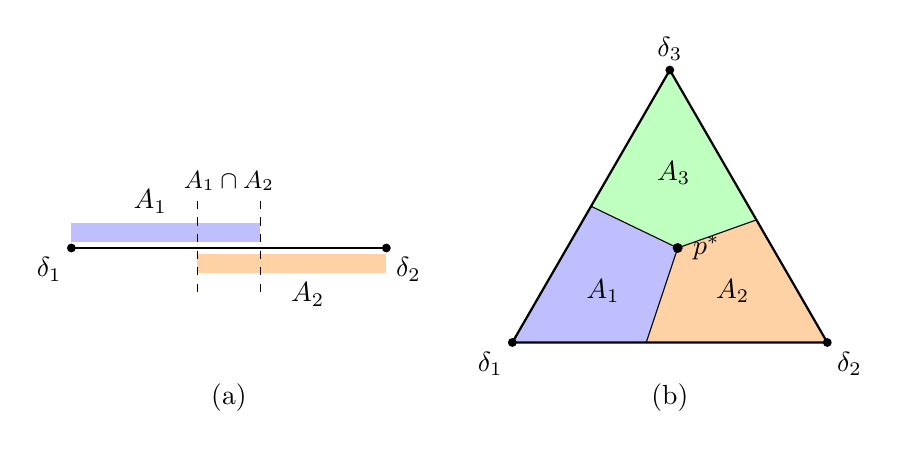
\begin{tikzpicture}
\begin{scope}[yshift=1.2cm]
 \fill[blue!25] (0,0.08) rectangle (2.4,0.32);
 \fill[orange!35] (1.6,-0.32) rectangle (4,-0.08);
 \draw[thick] (0,0) -- (4,0);
 \fill (0,0) circle (1.6pt); \fill (4,0) circle (1.6pt);
 \node[below left] at (0,0) {$\delta_1$};
 \node[below right] at (4,0) {$\delta_2$};
 \node[above] at (1.0,0.32) {$A_1$};
 \node[below] at (3.0,-0.32) {$A_2$};
 \draw[dashed] (1.6,0.6) -- (1.6,-0.6);
 \draw[dashed] (2.4,0.6) -- (2.4,-0.6);
 \node[above] at (2,0.6) {\small $A_1\cap A_2$};
 \node at (2,-1.9) {(a)};
\end{scope}
\begin{scope}[xshift=5.6cm]
 \coordinate (d1) at (0,0); \coordinate (d2) at (4,0); \coordinate (d3) at (2,3.46);
 \coordinate (e12) at (1.7,0); \coordinate (e23) at (3.1,1.557); \coordinate (e13) at (1,1.73);
 \coordinate (c) at (2.1,1.2);
 \fill[blue!25] (d1)--(e12)--(c)--(e13)--cycle;
 \fill[orange!35] (d2)--(e23)--(c)--(e12)--cycle;
 \fill[green!25] (d3)--(e13)--(c)--(e23)--cycle;
 \draw[thick] (d1)--(d2)--(d3)--cycle;
 \draw (e12)--(c) (e23)--(c) (e13)--(c);
 \foreach \p in {d1,d2,d3} \fill (\p) circle (1.6pt);
 \node[below left] at (d1) {$\delta_1$};
 \node[below right] at (d2) {$\delta_2$};
 \node[above] at (d3) {$\delta_3$};
 \node at (1.15,0.65) {$A_1$};
 \node at (2.8,0.65) {$A_2$};
 \node at (2.05,2.15) {$A_3$};
 \fill (c) circle (1.8pt) node[right=2pt] {$p^*$};
 \node at (2,-0.7) {(b)};
\end{scope}
\end{tikzpicture}
\caption{Lemma~\ref{lem:kkm} for $|F|=2$ and $|F|=3$. Each vertex $\delta_\omega$ lies in $A_\omega$, and each face of the simplex is covered by the sets indexed by its vertices. (a)~Closed sets $A_1\ni\delta_1$ and $A_2\ni\delta_2$ that cover the segment must meet. (b)~Each edge is covered by the two sets of its endpoints; the three closed sets have a common point $p^*$.}
\label{fig:kkm}
\end{figure}

\begin{theorem}\label{thm:bayes-finite}
Let $\Omega$ be finite and let the ranking be generated by a loss $L:\M_L\times\Omega\to[0,\infty]$. Suppose that to each prior $p\in\Delta$ is assigned an undominated coherent model $c_p$ such that:
\begin{enumerate}[label=(\roman*)]
\item \emph{Bayes choice}: $c_p$ is a Bayes model for some prior whose support lies within $\supp p$; and
\item \emph{lower semicontinuity}: for each world $\omega$, the loss $L(c_p,\omega)$ is a lower semicontinuous function of $p$ on $\Delta$.
\end{enumerate}
Then every model is weakly dominated by one of the assigned models. If, in addition, every model with the same loss profile as an undominated coherent model is coherent, then the undominated models are exactly the undominated coherent ones, and every other model is dominated by an undominated coherent model.
\end{theorem}
\begin{proof}
Fix a model $m$. For each world $\omega$ let $A_\omega\coloneqq\{p\in\Delta:L(c_p,\omega)\le L(m,\omega)\}$. This set is all of $\Delta$ if $L(m,\omega)=\infty$, and otherwise a sublevel set of a lower semicontinuous function; either way it is closed. Let $p\in\Delta$. By (i) and Lemma~\ref{lem:bayes-competitive}, $c_p$ is competitive on $\supp p$, so some $\omega\in\supp p$ has $p\in A_\omega$. Lemma~\ref{lem:kkm} gives $p^*$ in every $A_\omega$, and then $L(c_{p^*})\le L(m)$. For the last claim, a model with the same profile as some $c\in\C_L$ is undominated, since a dominator of it would dominate $c$; so the additional hypothesis is closure under ties, and Proposition~\ref{prop:conclusion}(a) applies.
\end{proof}

Three features of the hypotheses matter in applications. The prior in (i) may differ from $p$ and need not vary continuously with it; Example~\ref{ex:conditional} shows that this freedom is needed. The assignment $p\mapsto c_p$ need not be continuous; only its losses must be lower semicontinuous. And the Bayes property is required only of the assigned models, not of every Bayes model. Figure~\ref{fig:profiles} illustrates the theorem, and shows what goes wrong without lower semicontinuity.

\begin{figure}[ht]
\centering
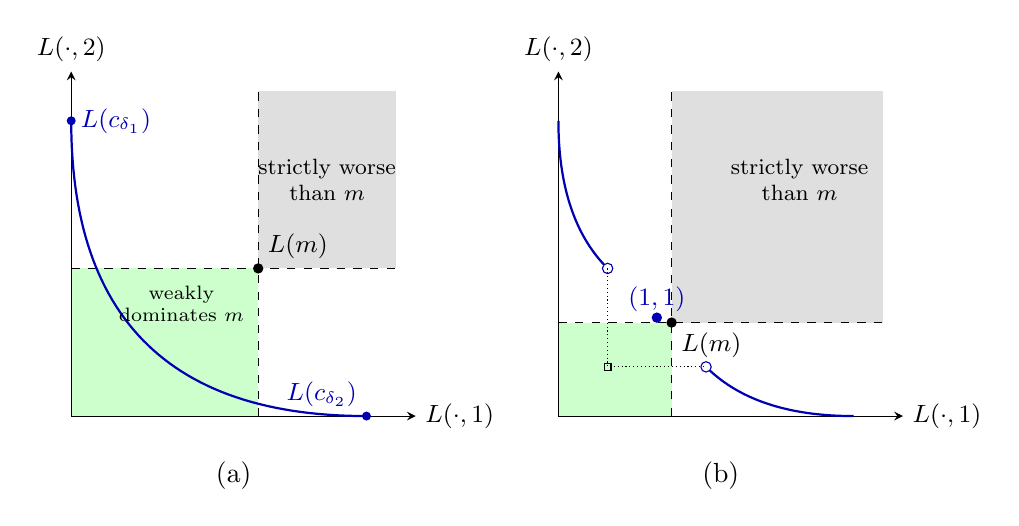
\begin{tikzpicture}[scale=1.25,>=stealth]
\begin{scope}
 \fill[gray!25] (1.9,1.5) rectangle (3.3,3.3);
 \fill[green!20] (0,0) rectangle (1.9,1.5);
 \draw[->] (0,0) -- (3.5,0) node[right] {\small $L(\cdot,1)$};
 \draw[->] (0,0) -- (0,3.5) node[above] {\small $L(\cdot,2)$};
 \draw[dashed] (1.9,0) -- (1.9,3.3);
 \draw[dashed] (0,1.5) -- (3.3,1.5);
 \draw[thick,blue!70!black,domain=0:1,samples=60] plot ({3*(1-\x)^2},{3*\x^2});
 \fill[blue!70!black] (0,3) circle (1.3pt) node[right] {\small $L(c_{\delta_1})$};
 \fill[blue!70!black] (3,0) circle (1.3pt) node[above left] {\small $L(c_{\delta_2})$};
 \fill (1.9,1.5) circle (1.5pt) node[above right] {\small $L(m)$};
 \node[align=center,font=\footnotesize] at (2.6,2.4) {strictly worse\\than $m$};
 \node[align=center,font=\scriptsize] at (1.12,1.14) {weakly\\dominates $m$};
 \node at (1.65,-0.6) {(a)};
\end{scope}
\begin{scope}[xshift=4.95cm]
 \fill[gray!25] (1.15,0.95) rectangle (3.3,3.3);
 \fill[green!20] (0,0) rectangle (1.15,0.95);
 \draw[->] (0,0) -- (3.5,0) node[right] {\small $L(\cdot,1)$};
 \draw[->] (0,0) -- (0,3.5) node[above] {\small $L(\cdot,2)$};
 \draw[dashed] (1.15,0) -- (1.15,3.3);
 \draw[dashed] (0,0.95) -- (3.3,0.95);
 \draw[thick,blue!70!black,domain=0.5:1,samples=40] plot ({2*(1-\x)^2},{1+2*\x^2});
 \draw[thick,blue!70!black,domain=0:0.5,samples=40] plot ({1+2*(1-\x)^2},{2*\x^2});
 \draw[blue!70!black,fill=white] (0.5,1.5) circle (1.5pt);
 \draw[blue!70!black,fill=white] (1.5,0.5) circle (1.5pt);
 \fill[blue!70!black] (1,1) circle (1.5pt) node[above,inner sep=2pt] {\small $(1,1)$};
 \fill (1.15,0.95) circle (1.5pt) node[below right] {\small $L(m)$};
 \draw[densely dotted] (0.5,1.5) -- (0.5,0.5) -- (1.5,0.5);
 \draw (0.5,0.5) node[draw,rectangle,inner sep=1.2pt] {};
 \node[align=center,font=\footnotesize] at (2.45,2.4) {strictly worse\\than $m$};
 \node at (1.65,-0.6) {(b)};
\end{scope}
\end{tikzpicture}
\caption{(a)~Theorem~\ref{thm:bayes-finite} for two worlds. The assigned profiles $p\mapsto L(c_p)$ run from $L(c_{\delta_1})$, left of the vertical dashed line, to $L(c_{\delta_2})$, below the horizontal one. The sets $A_1$ and $A_2$ in the proof consist of the priors whose assigned profiles lie left of, respectively below, these lines. Every assigned model is competitive on $\supp p$, so the profiles avoid the grey quadrant of profiles strictly worse than $L(m)$; hence they meet the lower-left quadrant of profiles that weakly dominate $L(m)$. (b)~A discontinuous strictly proper score of the kind in Example~4 of Schervish, Seidenfeld and Kadane~\cite{SSK09}. A forecast $f\in[0,1]^2$ of the events $\{1\}$ and $\{2\}$ has loss $s(1,f_i)+s(0,f_j)$ at world~$i$, where $j\ne i$, $s(1,x)\coloneqq(1-x)^2+\frac12\one\{x<\frac12\}+\frac14\one\{x=\frac12\}$ and $s(0,x)\coloneqq x^2+\frac12\one\{x>\frac12\}+\frac14\one\{x=\frac12\}$. Take $c_p\coloneqq p$ and $m\coloneqq(0.6,0.7)$, so $L(m)=(1.15,0.95)$. As $p$ passes through $(\frac12,\frac12)$, the assigned profiles jump from near $(0.5,1.5)$ to $(1,1)$ to near $(1.5,0.5)$. They avoid the grey quadrant but skip the lower-left one: no coherent model weakly dominates $m$. Lower semicontinuity fails; it would force the profile at $(\frac12,\frac12)$ to lie at or below the boxed corner $(0.5,0.5)$. Correspondingly, the set of priors whose assigned model does at least as well as $m$ at world~$2$ contains every $p$ with $p_1<\frac12$ but not $(\frac12,\frac12)$, so it is not closed.}
\label{fig:profiles}
\end{figure}

For infinitely many worlds there is no simplex of priors on all worlds. We work on finite sets of worlds and join them by compactness. A space is compact if every open cover has a finite subcover; no separation property is needed.

\begin{theorem}\label{thm:bayes-infinite}
Let $\Omega$ be any nonempty set and let the ranking be generated by a loss $L:\M_L\times\Omega\to[0,\infty]$. Suppose there are a compact space $\Theta$ and, for each $\theta\in\Theta$, an undominated coherent model $c_\theta$, such that:
\begin{enumerate}[label=(\roman*)]
\item \emph{lower semicontinuity}: for each world $\omega$, the map $\theta\mapsto L(c_\theta,\omega)$ is lower semicontinuous on $\Theta$; and
\item \emph{continuous Bayes choices on finite sets of worlds}: every finite set of worlds is contained in a nonempty finite set $F$ of worlds for which there is a continuous map $\sigma_F:\Delta_F\to\Theta$ such that each $c_{\sigma_F(p)}$ is a Bayes model for some prior whose support lies within $\supp p$.
\end{enumerate}
Then every model is weakly dominated by some $c_\theta$. With the additional hypothesis of Theorem~\ref{thm:bayes-finite}, its last conclusion follows.
\end{theorem}
We call the sets $F$ in (ii) \emph{linked}. Every world lies in a linked set, and every finite union of linked sets lies in a linked set.
\begin{proof}
Fix a model $m$. For each linked $F$, the set $T_F\coloneqq\{\theta:L(c_\theta,\omega)\le L(m,\omega)\text{ for all }\omega\in F\}$ is closed, by (i). For $\omega\in F$, the set $A_\omega\coloneqq\{p\in\Delta_F:L(c_{\sigma_F(p)},\omega)\le L(m,\omega)\}$ is closed, by (i) and the continuity of $\sigma_F$. By (ii) and Lemma~\ref{lem:bayes-competitive}, every $p\in\Delta_F$ lies in $A_\omega$ for some $\omega\in\supp p$. Lemma~\ref{lem:kkm} gives $p_F$ in every $A_\omega$, so $\sigma_F(p_F)\in T_F$, and $T_F\ne\varnothing$. Given linked sets $F_1,\dots,F_k$, choose a linked $G\supseteq F_1\cup\dots\cup F_k$; then $\varnothing\ne T_G\subseteq T_{F_1}\cap\dots\cap T_{F_k}$. So the closed sets $T_F$ have the finite intersection property, and compactness gives $\theta^*$ in all of them. Every world lies in some linked $F$, so $L(c_{\theta^*})\le L(m)$. The last claim follows as in Theorem~\ref{thm:bayes-finite}.
\end{proof}

When $\Omega$ is finite, $\Omega$ is itself linked, since it lies in a linked subset of itself. Theorem~\ref{thm:bayes-infinite} then reduces to Theorem~\ref{thm:bayes-finite}: given the data of Theorem~\ref{thm:bayes-finite}, take $\Theta\coloneqq\Delta$ and $\sigma_\Omega$ the identity; conversely, put $c_p\coloneqq c_{\sigma_\Omega(p)}$, whose losses are lower semicontinuous in $p$ because $\{p:L(c_{\sigma_\Omega(p)},\omega)\le a\}$ is the inverse image of a closed set under a continuous map. Theorem~\ref{thm:bayes-infinite} places no topological requirement on the set of coherent models or their loss profiles; in Proposition~\ref{prop:countable} the coherent loss profiles do not form a closed set.

The compact family cannot be dropped, even for a complete and transitive ranking. The following is the main example of the paper.

\begin{example}\label{ex:main}
Let $\Omega\coloneqq\{1,2,3,\dots\}$. The models are coherent models $e_n$ ($n\ge1$) and one incoherent model $x$, with
\[
L(e_n,\omega)\coloneqq\begin{cases}0,&\omega\le n,\\ 2+n,&\omega>n,\end{cases}\qquad L(x,\omega)\coloneqq1.
\]
For $n<k$, $e_k$ does better than $e_n$ at the worlds $n<\omega\le k$ and worse at the worlds $\omega>k$; so no $e_n$ weakly dominates another. And $x$ does worse than every $e_n$ at world~$1$. So every $e_n$ is undominated, and these are the undominated coherent models. No $e_n$ weakly dominates $x$, since $L(e_n,n+1)=2+n>1$. So $x$ is undominated and incoherent, and the dominance conclusion fails. Distinct models are never tied, so closure under ties holds.

Yet every hypothesis of Theorem~\ref{thm:bayes-infinite} holds except compactness. Take $\Theta\coloneqq\{1,2,3,\dots\}$ with the discrete topology and $c_n\coloneqq e_n$, so (i) holds trivially. Let every finite nonempty $F$ be linked, with $\sigma_F$ constant at $\max F$. The model $e_{\max F}$ has loss $0$ throughout $F$, so it is a Bayes model for every prior on $F$, and at least as good as every model at every world of $F$. The models that win on finite sets have no limit among the models: such a limit would have loss $0$ at every world. The losses beyond $n$ may be bounded; for instance, $3-1/n$ in place of $2+n$ gives the same conclusions.
\end{example}

\section{The general theorems}\label{sec:general}

The proofs of Theorems~\ref{thm:bayes-finite} and~\ref{thm:bayes-infinite} use the losses in two ways only. Lower semicontinuity makes the comparisons of the assigned models with a rival vary in a closed way, and Bayes choices make every rival matched at some charged world. This section isolates that mechanism for arbitrary rankings.

\subsection{Finitely many worlds}
\begin{theorem}\label{thm:finite}
Let $\Omega$ be finite and let $L$ be any ranking. Suppose that to each prior $p\in\Delta$ is assigned an undominated coherent model $c_p$, the same model whichever rival it is compared with. Suppose also that to each model $m$ and world $\omega$ is assigned a closed set $A_\omega(m)\subseteq\Delta$ such that:
\begin{enumerate}[label=(\roman*)]
\item \emph{guarantee}: $c_p\preceq_\omega m$ for every $p\in A_\omega(m)$;
\item \emph{every prior is served at a world it charges}: for every model $m$, every prior $p$ lies in $A_\omega(m)$ for some world $\omega$ that $p$ charges.
\end{enumerate}
Then:
\begin{enumerate}[label=(\alph*)]
\item for each model $m$, some prior lies in every $A_\omega(m)$, and the model assigned to any such prior weakly dominates $m$;
\item every undominated model is tied at every world with an undominated coherent model;
\item if closure under ties holds, the undominated models are exactly the undominated coherent ones, and every other model is dominated by one of them.
\end{enumerate}
\end{theorem}
\begin{proof}
(a) Fix $m$. The closed sets $A_\omega(m)$ satisfy the hypothesis of Lemma~\ref{lem:kkm}, by (ii), so some $p^*$ lies in all of them. By (i), $c_{p^*}\preceq_\omega m$ at every world. Parts (b) and (c) follow by Proposition~\ref{prop:conclusion}(a).
\end{proof}

The proof uses no property of the relations, no topology on models, no parametrisation of the coherent models and no numerical values. We read $A_\omega(m)$ as the set of priors at which the comparison with $m$ at $\omega$ is \emph{guaranteed}. The assigned model may make further comparisons that are not guaranteed, and it may jump as $p$ varies; only the guaranteed comparisons must vary in a closed way. What cannot be relaxed is that one assigned model serves against every rival at once (Remark~\ref{rem:collapse}). A simpler special case takes every comparison of the assigned model to be guaranteed.

\begin{corollary}\label{cor:closed-choice}
Let $\Omega$ be finite. Suppose that to each prior $p$ is assigned an undominated coherent model $c_p$, competitive on $\supp p$, such that each set $\{p:c_p\preceq_\omega m\}$ is closed. Then the conclusions of Theorem~\ref{thm:finite} hold.
\end{corollary}
\begin{proof}
Take $A_\omega(m)\coloneqq\{p:c_p\preceq_\omega m\}$. The guarantee holds by definition, and the serving condition (ii) is competitiveness.
\end{proof}

Theorem~\ref{thm:bayes-finite} is the case of Corollary~\ref{cor:closed-choice} for loss rankings in which closedness comes from lower semicontinuity and competitiveness from Lemma~\ref{lem:bayes-competitive}; its proof above is this argument. Competitiveness, and the serving condition, cannot be weakened to the requirement that no model strictly dominate the assigned model on $\supp p$:

\begin{example}\label{ex:incomparable}
Take one world, $\M_L\coloneqq\{a,b\}$ with $a$ and $b$ incomparable, and $\C\coloneqq\{a\}$. Then $\C_L=\{a\}$ and no model strictly dominates $a$. But $b$ is undominated and is weakly dominated by no coherent model.
\end{example}

Theorem~\ref{thm:finite} is strictly more general than Corollary~\ref{cor:closed-choice}. In the next example the assigned models must jump in a way that no closed full comparison sets allow.

\begin{example}\label{ex:two-world}
Let $\Omega\coloneqq\{1,2\}$. The models are coherent models $c_t$ and incoherent models $x_t$, for $t\in[0,1]$, with losses $(t,1-t)$ for $c_t$ and $(2,2)$ for $x_t$. At each world, accept every comparison $m\preceq_\omega m'$ in which the loss of $m$ at $\omega$ is at most that of $m'$, except $c_q\preceq_1x_q$ for $q>0$ and $c_0\preceq_2x_0$. The relations are reflexive but not transitive: for $0<q<s$, $c_q\preceq_1c_s\preceq_1x_q$, but not $c_q\preceq_1x_q$.

\emph{Dominance facts.} A weak dominator of $c_t$ has losses at most $(t,1-t)$, so it is $c_t$; hence $\C_L=\{c_t:t\in[0,1]\}$. Each $x_q$ is strictly dominated by every $c_s$ with $s\ne q$. So the dominance conclusion and closure under ties hold.

\emph{Theorem~\ref{thm:finite} applies.} Writing $p=(p_1,p_2)$, assign $c_{p_2}$ to $p$, and guarantee: against $c_s$, world~$1$ when $p_2\le s$ and world~$2$ when $p_2\ge s$; against $x_q$ with $q>0$, world~$1$ when $p_2=0$ and world~$2$ always; against $x_0$, world~$1$ always and world~$2$ when $p_2=1$. These sets are closed, and the guarantees hold by inspection. For the serving condition: if $p_2\le s$ and $p$ does not charge world~$1$, then $p=\delta_2$, so $s=1$ and world~$2$ is charged with $p_2\ge s$; the case $p_2\ge s$ is symmetric. Against $x_q$ with $q>0$, either world~$2$ is charged or $p=\delta_1$ and $p_2=0$; against $x_0$, either world~$1$ is charged or $p=\delta_2$.

\emph{Corollary~\ref{cor:closed-choice} fails for every assignment.} Suppose $p\mapsto c_p$ satisfied it. For $q>0$, only $c_q$ fails to be at least as good as $x_q$ at world~$1$, so $\{p:c_p\preceq_1x_q\}$ is the complement of $\{p:c_p=c_q\}$. Likewise $\{p:c_p\preceq_2x_0\}$ is the complement of $\{p:c_p=c_0\}$. These sets are closed, so every set $\{p:c_p=c_t\}$ is open. They partition the connected set $\Delta$, so the assignment is constant. But competitiveness at $\delta_1$ forces $c_0$, the only model at least as good as every model at world~$1$, and at $\delta_2$ it forces $c_1$.
\end{example}

Theorem~\ref{thm:finite} is also strictly more general than Theorem~\ref{thm:bayes-finite} for loss rankings, because Bayes choices are not preserved by rescaling (Lemma~\ref{lem:rescale}). The same example shows why the randomised complete class theorem does not settle our question.

\begin{example}\label{ex:rescale}
Take two worlds, $\M_L\coloneqq[0,1]^2$, $\C\coloneqq\{c:c_1+c_2=1\}$, and the quadratic losses $L_1(c)\coloneqq(1-c_1)^2+c_2^2$ and $L_2(c)\coloneqq c_1^2+(1-c_2)^2$. Writing $c=(s+k,1-s+k)$ with $s\in[0,1]$, the profile of $c$ is $(2(1-s)^2+2k^2,\ 2s^2+2k^2)$. So the coherent profiles ($k=0$) are pairwise incomparable, every incoherent model is strictly dominated by its coherent counterpart $(s,1-s)$, the undominated models are exactly the coherent ones, and closure under ties holds. Now rescale by $t\mapsto t^{1/4}$ at both worlds. Writing $a\coloneqq2^{1/4}$, the coherent profiles become $a(\sqrt{1-s},\sqrt s)$.

\emph{Corollary~\ref{cor:closed-choice} applies to the rescaled loss.} Under the quadratic loss, the assignment $p\mapsto(p_1,p_2)$ makes each assigned model a Bayes model for $p$ with continuous losses, so the hypotheses of Corollary~\ref{cor:closed-choice} hold, as in the proof of Theorem~\ref{thm:bayes-finite}. They refer only to the ranking, so they hold for the rescaled loss by Lemma~\ref{lem:rescale}.

\emph{Theorem~\ref{thm:bayes-finite} does not apply to it.} For a prior charging both worlds, the expected loss along the coherent arc, $a(p_1\sqrt{1-s}+p_2\sqrt s)$, is strictly concave in $s$, so its only coherent minimisers are the endpoints $(1,0)$ and $(0,1)$. Incoherent models are never Bayes models, since each is strictly dominated. So an assignment satisfying (i) takes only the values $(1,0)$ and $(0,1)$, with $(1,0)$ at $\delta_1$ and $(0,1)$ at $\delta_2$. By (ii), $\{p:c_p=(1,0)\}=\{p:L(c_p,1)\le0\}$ and $\{p:c_p=(0,1)\}$ are closed. They are disjoint, nonempty and cover $\Delta$, contradicting connectedness.

\emph{Randomisation.} Choosing at random among finitely many models yields the convex hull of their profiles. The coherent profiles lie on the arc $x^2+y^2=a^2$ and satisfy $x+y=a(\sqrt{1-s}+\sqrt s)\ge a$, with equality only at the endpoints; incoherent profiles lie above coherent ones. So every point of the convex hull lies on or above the line $x+y=a$, and the points of the segment from $(a,0)$ to $(0,a)$, which are mixtures of the endpoint profiles, are undominated among randomised profiles. Every other point $z$ of the hull has $z_1+z_2>a$ and coordinates in $[0,a]$, since the quadratic losses are at most $2=a^4$; so $z-\frac{z_1+z_2-a}{2}(1,1)$ lies on the segment and strictly below $z$. Hence the undominated randomised profiles are exactly the segment, and they share only the endpoints with the undominated original profiles. Moreover no original profile lies weakly below $(a/2,a/2)$: a coherent one would need $\sqrt{1-s}\le\frac12$ and $\sqrt s\le\frac12$, which is impossible, and an incoherent one would have a coherent one below it. So a randomised dominator need not be matched by any original model, and the randomised complete class theorem~\cite[Theorem~1]{SSSK}, which concerns the enlarged class, does not by itself identify the undominated original models.
\end{example}

\subsection{Arbitrary sets of worlds}
\begin{theorem}\label{thm:local}
Let $\Omega$ be any nonempty set and $L$ any ranking. Suppose:
\begin{enumerate}[label=\arabic*.,leftmargin=*]
\item \emph{A compact family of undominated coherent models with closed guaranteed comparisons.} There are a compact space $\Theta$ and, for each $\theta\in\Theta$, an undominated coherent model $c_\theta$. For each world $\omega$ and model $m$ there is a closed set $K_\omega(m)\subseteq\Theta$ such that $c_\theta\preceq_\omega m$ for every $\theta\in K_\omega(m)$.
\item \emph{Local guarantees on finite sets of worlds.} Every finite set of worlds is contained in a nonempty finite set $F$ of worlds, called \emph{linked}, for which there are a map $\theta_F:\Delta_F\to\Theta$, not necessarily continuous and the same for every rival, and for each $\omega\in F$ and model $m$ a closed set $A^F_\omega(m)\subseteq\Delta_F$, such that:
\begin{enumerate}[label=(\alph*)]
\item the local guarantees are global guarantees: $\theta_F(p)\in K_\omega(m)$ whenever $p\in A^F_\omega(m)$;
\item every prior is served at a world it charges: for every model $m$, every $p\in\Delta_F$ lies in $A^F_\omega(m)$ for some world $\omega$ that $p$ charges.
\end{enumerate}
\end{enumerate}
Then every model is weakly dominated by some $c_\theta$, and conclusions (b) and (c) of Theorem~\ref{thm:finite} hold.
\end{theorem}
In words: on each finite set of worlds, every prior is assigned one member of a fixed compact family of undominated coherent models, and this one member must serve against every rival. For each rival and world, the priors at which the comparison is guaranteed form a closed set, and every rival is guaranteed at some world that the prior charges, so that every prior is served at a world it charges. In the compact family, the members guaranteed to match or beat a given rival at a given world also form a closed set. Then a single member of the family matches or beats the rival at every world.
\begin{proof}
Fix a model $m$. For each linked $F$, the closed sets $A^F_\omega(m)$, $\omega\in F$, satisfy the hypothesis of Lemma~\ref{lem:kkm}, by (b). So some $p_F$ lies in all of them, and by (a), $\theta_F(p_F)\in\bigcap_{\omega\in F}K_\omega(m)$. Given worlds $\omega_1,\dots,\omega_k$, choose a linked $F$ containing them; then $\bigcap_iK_{\omega_i}(m)\supseteq\bigcap_{\omega\in F}K_\omega(m)\ni\theta_F(p_F)$. So the closed sets $K_\omega(m)$, $\omega\in\Omega$, have the finite intersection property. By compactness some $\theta^*$ lies in all of them, and $c_{\theta^*}\preceq_\omega m$ at every world. The rest is Proposition~\ref{prop:conclusion}(a).
\end{proof}

If each $\theta_F$ is continuous, conditions (a) and (b) may be replaced by one requirement: for every model $m$ and every $p\in\Delta_F$, some world $\omega$ charged by $p$ has $\theta_F(p)\in K_\omega(m)$. For then $A^F_\omega(m)\coloneqq\theta_F^{-1}(K_\omega(m))$ is closed. Theorem~\ref{thm:bayes-infinite} is the case $K_\omega(m)\coloneqq\{\theta:L(c_\theta,\omega)\le L(m,\omega)\}$ and $\theta_F\coloneqq\sigma_F$, with the requirement supplied by Lemma~\ref{lem:bayes-competitive}. For finitely many worlds nothing is lost relative to Theorem~\ref{thm:finite}: $\Omega$ is then linked, and its data give those of Theorem~\ref{thm:finite} with $c_p\coloneqq c_{\theta_\Omega(p)}$ and $A_\omega(m)\coloneqq A^\Omega_\omega(m)$; conversely, the data of Theorem~\ref{thm:finite} give those of Theorem~\ref{thm:local} with $\Theta\coloneqq\Delta$, $K_\omega(m)\coloneqq A_\omega(m)$, $\Omega$ as the only linked set, $\theta_\Omega$ the identity and $A^\Omega_\omega(m)\coloneqq A_\omega(m)$.

The next two remarks locate the content of Theorems~\ref{thm:finite} and~\ref{thm:local}.

\begin{remark}\label{rem:collapse}
Two natural weakenings are equivalent to the conclusion they would be used to prove. Suppose the dominance conclusion holds, and choose, using the axiom of choice, an undominated coherent model $d(m)$ weakly dominating each model $m$. Give $\C_L$, which is nonempty, the cofinite topology, whose closed sets are the finite sets and $\C_L$ itself. It is compact, since a nonempty member of an open cover has finite complement, which finitely many further members cover. Put $c_\theta\coloneqq\theta$ and $K_\omega(m)\coloneqq\{d(m)\}$, which is closed.
\begin{enumerate}[label=(\roman*)]
\item \emph{An assigned model that may depend on the rival.} If each rival $m$ could have its own assignment, the hypotheses would then hold: assign $d(m)$ to every prior when $m$ is the rival, and let every set of priors at which the comparison with $m$ is guaranteed be the whole simplex.
\item \emph{An abstract compactness condition.} Suppose we asked only for item~1 of Theorem~\ref{thm:local}, together with: for each model $m$ and finite set of worlds, some single $\theta$ is guaranteed against $m$ at every world of that set. The finite-intersection and compactness argument in the proof of Theorem~\ref{thm:local} derives the dominance conclusion from this condition, and the family just defined satisfies it whenever the conclusion holds. So the condition is equivalent to the conclusion. Requiring $\Theta$ to be Hausdorff changes nothing: the one-point compactification of the discrete space $\C_L$, with any member of $\C_L$ at the added point, serves equally, since its singletons are closed.
\end{enumerate}
So neither condition explains why dominance holds. The content of the theorems lies in one assigned model per prior, serving against every rival at once, with guarantees that are closed in the prior.
\end{remark}

\begin{remark}\label{rem:vertex}
Conversely, the hypotheses of Theorems~\ref{thm:finite} and~\ref{thm:local} are not implied by the dominance conclusion. At a vertex $\delta_\omega$, the serving condition forces $\delta_\omega$ into the guarantee set at $\omega$ of every rival. So the hypotheses imply that at every world some undominated coherent model is at least as good as every model. That fails for the loss ranking with two worlds whose models, all coherent, have the profiles $(t,1-t)$ for $t\in(0,1]$. These profiles are pairwise incomparable, so every model is undominated and the dominance conclusion holds trivially; but no model has loss $0$ at world~$1$.
\end{remark}

\emph{Guarantees on finite sets of worlds need a compact family to link them.} Say that a ranking has \emph{guarantees on a finite set $G$ of worlds} if the data of Theorem~\ref{thm:finite} exist for the worlds of $G$: an assigned model for each prior on $G$, and closed sets of priors on $G$ satisfying the guarantee and the serving condition, with the assigned models taken from the undominated coherent models of the ranking on all of $\Omega$. The hypotheses of Theorem~\ref{thm:local} give guarantees on every finite set $G$: choose a linked $F\supseteq G$, restrict to the priors on $G$, assign $c_{\theta_F(p)}$, and use the sets $A^F_\omega(m)\cap\Delta_G$ for $\omega\in G$; the serving condition survives because a prior on $G$ charges only worlds of $G$. In Example~\ref{ex:main} there are guarantees on every finite set of worlds: assign $e_{\max G}$ to every prior on $G$ and guarantee every comparison. Yet the dominance conclusion fails. So guarantees on finite sets of worlds do not suffice without a compact family linking them.

\begin{remark}\label{rem:closed-comparisons}
Suppose every comparison the compact family makes has closed sections: $\{\theta:c_\theta\preceq_\omega m\}$ is closed for every world $\omega$ and model $m$. For loss rankings this holds when the losses along the family are lower semicontinuous. Then item~1 of Theorem~\ref{thm:local} holds with $K_\omega(m)$ taken to be these sets, and item~2(a) says only that the model assigned to $p$ is at least as good as $m$ at $\omega$ whenever $p\in A^F_\omega(m)$. Every application in Section~\ref{sec:apps} meets the hypotheses in this form, which is why none of them needs more than Theorem~\ref{thm:bayes-infinite}. The requirement is not necessary. In Example~\ref{ex:two-world}, Theorem~\ref{thm:local} applies, since for finitely many worlds its hypotheses are those of Theorem~\ref{thm:finite}. But no compact family whose full comparison sets are closed meets the hypotheses of Theorem~\ref{thm:local}. By its conclusion such a family contains a weak dominator of each $c_t$, which is $c_t$ itself, so every set $E_t\coloneqq\{\theta:c_\theta=c_t\}$ is nonempty. The full comparison sets against $x_q$ ($q>0$) at world~$1$, and against $x_0$ at world~$2$, are the complements of the $E_t$. If they were closed, the $E_t$ would be infinitely many disjoint nonempty open sets covering a compact space, which is impossible. Copying each world infinitely often gives the same phenomenon on an infinite set of worlds, with $\theta_F(p)$ the probability that $p$ gives to copies of world~$2$.
\end{remark}

The results of the next section need more: lower semicontinuous losses along the family. This is stronger than closed comparison sets, and it supplies comparisons with arbitrary numerical bounds, not only with the losses of models.

\section{Margins, Bayes models and strict dominance}\label{sec:margins}
These results use the numerical values of the losses. Their hypotheses are exactly those of Theorem~\ref{thm:bayes-infinite}.

\begin{theorem}\label{thm:margin}
Assume the hypotheses of Theorem~\ref{thm:bayes-infinite}. For $x:\Omega\to(-\infty,\infty]$, with $\pi\cdot x$ defined as for losses, the following are equivalent:
\begin{enumerate}[label=(\alph*)]
\item some model $m$ has $L(m,\omega)\le x(\omega)$ at every world;
\item some $c_\theta$ does;
\item $\pi\cdot x\ge V(\pi)$ for every finitely supported prior $\pi$.
\end{enumerate}
\end{theorem}
\begin{proof}
(b) implies (a) trivially, and (a) implies (c) since $V(\pi)\le\pi\cdot L(m)\le\pi\cdot x$. Assume (c), and fix a linked $F$. The sets $A_\omega\coloneqq\{p\in\Delta_F:L(c_{\sigma_F(p)},\omega)\le x(\omega)\}$, $\omega\in F$, are closed, by lower semicontinuity and the continuity of $\sigma_F$. Suppose some $p$ lies in no $A_\omega$ with $\omega\in\supp p$. Let $c\coloneqq c_{\sigma_F(p)}$ be a Bayes model for $\pi$, with $\supp\pi\subseteq\supp p$. Then $x(\omega)<L(c,\omega)$ on $\supp\pi$, so $x$ is finite there and $\pi\cdot x<\pi\cdot L(c)=V(\pi)$, contrary to (c). (If $\pi\cdot L(c)=\infty$ this is immediate.) So Lemma~\ref{lem:kkm} applies and gives some $\theta$ in $T_F\coloneqq\{\theta:L(c_\theta,\omega)\le x(\omega)\text{ for all }\omega\in F\}$, which is closed by lower semicontinuity. As in the proof of Theorem~\ref{thm:bayes-infinite}, the sets $T_F$ have the finite intersection property, and compactness gives $\theta$ in all of them.
\end{proof}

Take $x\coloneqq L(m)-\varepsilon$, with $\infty-\varepsilon\coloneqq\infty$. Then a model with finite losses is uniformly dominated by some model, or equivalently by some $c_\theta$, iff for some $\varepsilon>0$ its expected loss is at least $V(\pi)+\varepsilon$ for every finitely supported prior $\pi$. Theorem~\ref{thm:bayes-infinite} is the case $x=L(m)$.

\begin{corollary}\label{cor:bayes-exist}
Under the hypotheses of Theorem~\ref{thm:bayes-infinite}, every finitely supported prior $\pi$ has a Bayes model among the $c_\theta$.
\end{corollary}
\begin{proof}
The map $\theta\mapsto\pi\cdot L(c_\theta)$ is lower semicontinuous on the compact space $\Theta$, so it attains its infimum at some $\theta^*$: if the infimum is finite, the nonempty closed sets $\{\theta:\pi\cdot L(c_\theta)\le a\}$, for real $a$ above it, are nested, and compactness gives a point in all of them; otherwise every $\theta$ attains it. Every model $m$ is weakly dominated by some $c_\theta$, so $\pi\cdot L(c_{\theta^*})\le\pi\cdot L(m)$.
\end{proof}

\begin{proposition}\label{prop:strict}
Let $\Omega$ be finite and assume the hypotheses of Theorem~\ref{thm:bayes-finite}, which are those of Theorem~\ref{thm:bayes-infinite} with $\Theta\coloneqq\Delta$ and $\sigma_\Omega$ the identity. Suppose $V$ is upper semicontinuous on $\Delta$. This holds if
\begin{enumerate}[label=(\alph*)]
\item the assigned models have finite losses; or
\item $V$ is finite, each $c_p$ is a Bayes model for $p$ itself, and each $p\mapsto L(c_p,\omega)$ is continuous.
\end{enumerate}
Then a model is strictly dominated iff it is a Bayes model for no prior, and in that case some assigned model uniformly dominates it. In particular, if every Bayes model is an undominated coherent model, every other model is uniformly dominated by an undominated coherent model.
\end{proposition}
\begin{proof}
A strict dominator of $m$ has finite losses and smaller expected loss than $m$ under every prior, so $m$ is a Bayes model for no prior. Conversely, let $m$ be a Bayes model for no prior. Then $V$ is finite, since $V(\pi)=\infty$ would make every model a Bayes model for $\pi$. Let $\Omega_\infty\coloneqq\{\omega:L(m,\omega)=\infty\}$, and put $x_n(\omega)\coloneqq L(m,\omega)-1/n$ for $\omega\notin\Omega_\infty$ and $x_n(\omega)\coloneqq n$ for $\omega\in\Omega_\infty$. The functions $g_n(\pi)\coloneqq\pi\cdot x_n-V(\pi)$ are lower semicontinuous, since $x_n$ is finite and $V$ is finite and upper semicontinuous, and they increase with $n$. They tend to $\pi\cdot L(m)-V(\pi)>0$ when $\pi(\Omega_\infty)=0$, and to $\infty$ otherwise. So the closed sets $\{g_n\le0\}$ decrease and have empty intersection, and by compactness some $\{g_N\le0\}$ is empty. Theorem~\ref{thm:margin} with $x\coloneqq x_N$ gives an assigned model $c_p$ with $L(c_p)\le x_N$, which uniformly dominates $m$ with margin $1/N$. The last claim follows, since a model outside $\C_L$ is then a Bayes model for no prior.

Upper semicontinuity in case (a): every model is weakly dominated by an assigned model (Theorem~\ref{thm:bayes-finite}), so $V(\pi)=\inf_p\pi\cdot L(c_p)$, an infimum of continuous functions. In case (b), fix $p$ and $\varepsilon>0$. For an interior prior $q$, $V(q)$ is finite, so the Bayes model $c_q$ has finite losses and $\pi\mapsto\pi\cdot L(c_q)$ is continuous. As interior $q$ tend to $p$, $p\cdot L(c_q)\to p\cdot L(c_p)=V(p)$, by continuity of the losses, which are finite on $\supp p$. Choose such a $q$ with $p\cdot L(c_q)<V(p)+\varepsilon/2$. Then for $\pi$ near $p$, $V(\pi)\le\pi\cdot L(c_q)<V(p)+\varepsilon$.
\end{proof}

Without (a) or (b) the equivalence can fail.
\begin{example}\label{ex:ssk-sharp}
This is Example~2 of~\cite{SSK09}. Let $\Omega\coloneqq\{1,2\}$, $\M_L\coloneqq[0,1]^2$, $\C\coloneqq\{(t,1-t):0\le t\le1\}$, and
\[
L(f,1)\coloneqq(1-f_1)^2+g_0(f_2),\qquad L(f,2)\coloneqq f_1^2+g_1(f_2),
\]
where $g_0(0)\coloneqq0$, $g_0(y)\coloneqq1+y$ for $y>0$, $g_1(0)\coloneqq\infty$ and $g_1(y)\coloneqq y-\log y$ for $y>0$. The $p$-expected loss of $f$ is $p_1(1-f_1)^2+p_2f_1^2+p_1g_0(f_2)+p_2g_1(f_2)$. The first part has unique minimiser $f_1=p_1$. If $p_2=0$ the second part is $g_0(f_2)$, with unique minimiser $0$. If $p_2>0$, it is $\infty$ at $f_2=0$ and has derivative $1-p_2/f_2$ for $f_2>0$, so its unique minimiser is $p_2$. Hence $c_p\coloneqq p$ is the unique Bayes model for $p$, with $V(p)=p_1p_2+1-p_2\log p_2$ for $p_2>0$ and $V(\delta_1)=0$. Since $V$ is finite, a weak dominator of $c_p$ is a Bayes model for $p$, so it equals $c_p$; this gives $\C_L=\C$ and closure under ties. The losses $L(c_p,1)=p_2^2+g_0(p_2)$ and $L(c_p,2)=p_1^2+g_1(p_2)$ are lower semicontinuous, since $g_0$ jumps up only away from $0$. So Theorem~\ref{thm:bayes-finite} applies. Now $m\coloneqq(\frac12,0)$ has $L(m)=(\frac14,\infty)$, so $p\cdot L(m)>V(p)$ for every $p$, and $m$ is a Bayes model for no prior. The coherent model $(1,0)$, with profile $(0,\infty)$, dominates $m$. But $L(f,1)<\frac14$ forces $f_2=0$ and then $L(f,2)=\infty$, so no model strictly dominates $m$. Here (a) fails, since $(1,0)$ has infinite loss, and so does (b): $V(p)\to1$ as $p\to\delta_1$ with $p_2>0$, while $V(\delta_1)=0$.
\end{example}

\section{Constructing rankings}\label{sec:construct}
So far the ranking was given. One can instead start from the coherent class and build a ranking for which the dominance conclusion holds. Fix the worlds, a nonempty set $\M_L$ of models and the coherent class $\C$; in this section ``model'' means a member of $\M_L$, and ``coherent model'' a member of $\C\cap\M_L$.
\begin{itemize}[leftmargin=*]
\item To each ordered pair $(m,m')$ of models assign \emph{the change} from $m'$ to $m$. The change from a model to itself is the \emph{null change}; the change from $m'$ to $m$ is null only if $m=m'$.
\item A change is \emph{available to} a model $z$ if it is the change from $z$ to some model.
\item For each world $\omega$, fix a set of changes said to be \emph{guided at $\omega$} (by the truth there), containing the null change, and a real-valued \emph{score} $\varphi_\omega$ on models, larger being better.
\end{itemize}
Rank by: $m\preceq_\omega m'$ iff the change from $m'$ to $m$ is guided at $\omega$, or it is available to no coherent model and $\varphi_\omega(m)>\varphi_\omega(m')$. Thus a change is accepted if guidance endorses it; otherwise it is accepted only if it strictly improves the score and no coherent model could make it.

\begin{proposition}\label{prop:construct}
Consider the ranking just defined.
\begin{enumerate}[label=(\alph*)]
\item Each $\preceq_\omega$ is reflexive. Suppose \emph{guided changes improve the score}: every non-null change guided at $\omega$ strictly raises $\varphi_\omega$. Then $m\preceq_\omega m'$ with $m\ne m'$ implies $\varphi_\omega(m)>\varphi_\omega(m')$. Hence every cycle $m_0\preceq_\omega m_1\preceq_\omega\dots\preceq_\omega m_k\preceq_\omega m_0$ consists of equal models, and distinct models are never tied at $\omega$.
\item Suppose \emph{guidance protects coherent models}: for every coherent model $c$, the only model reached from $c$ by a change guided at every world is $c$ itself. Then no model other than $c$ weakly dominates a coherent model $c$. So every coherent model is an undominated coherent model.
\item Assume both conditions. Then the following are equivalent:
\begin{enumerate}[label=(\roman*)]
\item every model is weakly dominated by an undominated coherent model;
\item every incoherent model $m$ has a coherent model $c$ such that the change from $m$ to $c$ is either guided at every world, or available to no coherent model and raises the score at every world.
\end{enumerate}
When they hold, closure under ties holds, and every incoherent model is strictly dominated by an undominated coherent model.
\end{enumerate}
\end{proposition}
\begin{proof}
(a) The null change is guided, so each $\preceq_\omega$ is reflexive. For $m\ne m'$, an accepted change raises $\varphi_\omega$: on the guided branch by hypothesis, on the other by definition. Around a cycle the scores are therefore equal, so every step is between equal models.

(b) Let $m$ weakly dominate a coherent $c$. The change from $c$ to $m$ is available to the coherent model $c$, so it is accepted at each world only as a guided change. Protection gives $m=c$. A dominator of $c$ would weakly dominate $c$ and differ from it, since $c$ is tied with itself by reflexivity.

(c) Suppose (i), and let an undominated coherent $c$ weakly dominate an incoherent $m$. Then $c\ne m$, and at each world the change from $m$ to $c$ is guided or improving, so $\varphi_\omega(c)>\varphi_\omega(m)$ either way, by (a). Whether the change is available to a coherent model does not depend on the world. If it is available to none, it raises the score at every world; if it is available to one, it is accepted at every world only as a guided change. This gives (ii). Conversely, suppose (ii), and let $m$ and $c$ be as there. Then $c\preceq_\omega m$ at every world and $c\ne m$, so by (a) $m\preceq_\omega c$ fails at every world, and $c$ strictly dominates $m$. By (b), every coherent model is undominated and weakly dominates itself. This gives (i). Finally, a model tied with a coherent $c$ weakly dominates $c$, so it is $c$, by (b); this is closure under ties.
\end{proof}

When guided changes improve the score, the ranking is acyclic (Proposition~\ref{prop:construct}(a)); in general it is not transitive, and the companion paper gives an example on the full space of gambles in two dimensions~\cite{KCM}. So, of the consequences in Section~\ref{sec:conclusion}, those that use no order properties apply; the dominance conclusion itself comes from Proposition~\ref{prop:construct}(c), not from Section~\ref{sec:general}. Proposition~\ref{prop:construct} answers the third question directly. It does not pass through Bayes choices or compact families, and nothing requires a ranking built in this way to meet their hypotheses.

The proposition places no constraint on how changes are individuated. If every ordered pair of distinct models is its own change, a change is available to a coherent model exactly when it starts from one; every score improvement of an incoherent model is then accepted, and (c)(ii) asks only for a coherent model with a better score at every world. The construction has content when changes are individuated coarsely, so that one change is available to many models, and the comparison of two models at a world depends only on the change between them. Its substance then lies in the existence of the improvements in (c)(ii), which must be proved for each class of models.

In the companion paper, \emph{Coherence and accuracy for sets of desirable gambles}~\cite{KCM}, the change from one set of desirable gambles to another consists of the gambles added and the gambles removed. For a separable space of gambles containing the constants, with models identified up to null sets of a fixed measure on gambles that satisfies a finite-moment and a null-boundary condition, its repair theorem shows that every incoherent model can be replaced by a coherent one through a change that no coherent model could make and that raises the score at every world by a uniform margin; the ranking is obtained as a consequence. The construction uses the distinction between changes available and unavailable to coherent models. So it shows that a ranking can accept every guided comparison, accept comparisons between distinct models only when they raise the score, be closed under ties, and still have exactly the coherent models as its undominated models; it does not, by itself, derive coherence from independently justified comparisons of performance. The companion paper also shows that, for its score, this ranking is the largest relation that accepts every guided comparison, accepts comparisons between distinct models only when they raise the score, and accepts a change available to a coherent model only as guidance. The last requirement restricts individual comparisons at individual worlds, and it is stronger than coherent admissibility, which asks only that coherent models remain undominated; its independent justification is open.

\section{Applications}\label{sec:apps}
Each application has three steps: show that every coherent model is undominated, so that $\C_L=\C$; apply Theorem~\ref{thm:bayes-finite} or~\ref{thm:bayes-infinite} through an explicit assignment of Bayes models; and obtain uniform or strict dominance from Section~\ref{sec:margins}. This verifies the conditions for a single ranking. Coherent admissibility for a family holds when the losses considered jointly cover the intended coherent class.

\subsection{Proper scores on finite domains}\label{sec:proper}
\begin{proposition}\label{prop:proper}
Let $\Omega$ be finite and $\C=\Delta\subseteq\M_L$. Suppose each $p\mapsto L(p,\omega)$ is lower semicontinuous on $\Delta$, and $L$ is \emph{strictly proper relative to $\M_L$}: each $p$ is a Bayes model for $p$, and every Bayes model for $p$ has the profile $L(p)$. Then every coherent model is undominated, every model is weakly dominated by a coherent one, and the undominated models are exactly those with a coherent loss profile. If $p$ is the only Bayes model for $p$, for every $p$, then the undominated models are exactly the coherent ones, and every incoherent model is dominated by a coherent one. If moreover every probability has finite losses, or each $p\mapsto L(p,\omega)$ is continuous, then every incoherent model is uniformly dominated by a coherent one.
\end{proposition}
\begin{proof}
A weak dominator of $p$ is a Bayes model for $p$, so it has profile $L(p)$; hence no model dominates $p$, and $\C_L=\C$. Theorem~\ref{thm:bayes-finite} applies with $c_p\coloneqq p$, and Proposition~\ref{prop:profiles} identifies the undominated models. With unique Bayes models, a model with profile $L(p)$ is a Bayes model for $p$, hence equal to $p$; this is closure under ties, and no incoherent model is a Bayes model. For the last claim, suppose some model is incoherent. Then $V$ is finite, since $V(p)=\infty$ would make every model, including an incoherent one, a Bayes model for $p$. Proposition~\ref{prop:strict}, case (a) or (b), shows that every incoherent model, being a Bayes model for no prior, is uniformly dominated by some $p$.
\end{proof}

This contains Pettigrew's Theorem~1~\cite{Pettigrew}. There the models are the credence functions on all subsets of a finite $\Omega$, the probabilities among them correspond to the points of $\Delta$, expected losses are read with $0\cdot\infty=0$, and uniqueness and continuity on all credence functions are assumed. Continuity cannot simply be dropped~\cite{SSK09}; a discontinuous strictly proper score such as that of Figure~\ref{fig:profiles}(b) is not lower semicontinuous on the probabilities.

\emph{Event forecasts.} Predd et al.~\cite{Predd} fix events $E_1,\dots,E_n$ in a nonempty set $\Omega$ and a continuous score $s:\{0,1\}\times[0,1]\to[0,\infty]$. Forecasts $f\in[0,1]^n$ have loss $L(f,\omega)\coloneqq\sum_is(\one_{E_i}(\omega),f_i)$, and $f$ is coherent if $f=(\pi(E_i))_i$ for a probability $\pi$. Proposition~\ref{prop:proper} does not apply directly, since the coherent forecasts are not the priors, but Theorem~\ref{thm:bayes-finite} and Proposition~\ref{prop:strict} do. The loss depends on $\omega$ only through its truth-value pattern $\tau(\omega)\coloneqq(\one_{E_i}(\omega))_i$, so loss profiles on $\Omega$ and on the finite set $\tau(\Omega)$ determine each other, the dominance relations agree, and we may replace $\Omega$ by $\tau(\Omega)$. To a prior $p$ on $\tau(\Omega)$ assign $c_p\coloneqq(p(E_i))_i$, where $p(E_i)$ is the probability of the patterns with $i$th entry $1$; these are the coherent forecasts. The $p$-expected loss of $f$ is $\sum_iG_{p(E_i)}(f_i)$, where $G_t(y)\coloneqq ts(1,y)+(1-t)s(0,y)$. Call $s$ \emph{proper} if each $G_t$ is minimised at $t$, and \emph{strictly proper} if $t$ is its unique minimiser. If $s$ is strictly proper, the minimum of each $G_t$ is finite, since otherwise every $y$ would minimise it. So $c_p$ is the unique Bayes model for $p$, $V$ is finite, and no incoherent forecast is a Bayes model. A weak dominator of $c_p$ is then a Bayes model for $p$, so it equals $c_p$; this gives $\C_L=\C$ and closure under ties. Continuity of $s$ makes the losses along $c_p$ continuous. Theorem~\ref{thm:bayes-finite} and Proposition~\ref{prop:strict}(b) therefore show that every incoherent forecast is uniformly dominated by a coherent one, which is~\cite[Theorem~1]{Predd}. The same argument allows a different continuous score $s_i$ for each event that is merely proper, in the same sense with $s_i$ in place of $s$, with $s_i(0,y)<\infty$ for $y<1$ and $s_i(1,y)<\infty$ for $y>0$, normalised so that $s_i(0,0)=s_i(1,1)=0$. Then $c_p$ is a Bayes model for $p$ and $V$ is finite, and any other Bayes model $f$ has $L(f)=L(c_p)$~\cite[Lemma~5]{SSK09}. So $\C_L=\C$, although closure under ties may fail. Theorem~\ref{thm:bayes-finite} and Proposition~\ref{prop:profiles} show that the undominated forecasts are those with a coherent loss profile, and Proposition~\ref{prop:strict}(b) that every forecast that is a Bayes model for no prior is uniformly dominated by a coherent one. This is~\cite[Theorem~2, Conclusion~3]{SSK09} for unconditional forecasts.

\subsection{Probabilism on arbitrary domains}\label{sec:nielsen}
Let $\Omega$ be any nonempty set, $\M_L\coloneqq[0,1]^{2^\Omega}$ the credence functions on its subsets, and $\C$ the finitely additive probabilities. With the topology of pointwise convergence on subsets, $\C$ is compact, as a closed subset of a product of intervals; on $\C$ this is the weak-star topology, since bounded functions are uniform limits of simple ones. Let $L:\M_L\times\Omega\to[0,\infty]$. For $q\in\C$ and $f:\Omega\to[0,\infty]$, let $E_qf$ be the supremum of $q(h)$ over bounded $h\le f$, as in~\cite[Appendix~A]{Nielsen}.

\begin{theorem}\label{thm:nielsen}
Assume \emph{quasi-strict propriety}: $E_qL(q,\cdot)\le E_qL(m,\cdot)$ for every $q\in\C$ and $m\in\M_L$, strictly when $m\notin\C$. Assume also that $q\mapsto L(q,\omega)$ is lower semicontinuous on $\C$ for every world $\omega$. Then the undominated models are exactly the finitely additive probabilities, and every other model is dominated by one of them. If in addition each probability has bounded loss across worlds, every other model is uniformly dominated by a probability.
\end{theorem}
\begin{proof}
\emph{Every probability is undominated.} Suppose $L(m)\le L(q)$ with $q\in\C$ and $L(m,w)<L(q,w)$. Then $E_qL(m,\cdot)\le E_qL(q,\cdot)$, which is finite because quasi-strict propriety gives $E_qL(q,\cdot)<E_qL(m',\cdot)$ for any $m'\notin\C$, such as the zero credence function. So equality holds, and $L(m,w)$ is finite. For $n\ge2$ put $q_n\coloneqq\frac1n\delta_w+(1-\frac1n)q$. Expectations are linear in the probability~\cite[Appendix~A, Proposition~1]{Nielsen}, so quasi-strict propriety at $q_n$ and at $q$ gives
\[
\tfrac1nL(m,w)+(1-\tfrac1n)E_qL(q,\cdot)\ \ge\ \tfrac1nL(q_n,w)+(1-\tfrac1n)E_qL(q_n,\cdot)\ \ge\ \tfrac1nL(q_n,w)+(1-\tfrac1n)E_qL(q,\cdot),
\]
that is, $L(q_n,w)\le L(m,w)$. Since $q_n\to q$, lower semicontinuity gives $L(q,w)\le L(m,w)$, a contradiction. So $\C_L=\C$.

\emph{Theorem~\ref{thm:bayes-infinite} applies.} Take $\Theta\coloneqq\C$, $c_q\coloneqq q$, every finite nonempty set linked, and $\sigma_F(p)\coloneqq p$, viewed as a member of $\C$; this map is continuous. For finitely supported $p$ and $[0,\infty]$-valued $f$, $E_pf=\sum_\omega p_\omega f(\omega)$, by truncating $f$ at $n$ and letting $n\to\infty$. So quasi-strict propriety makes $p$ a Bayes model for $p$.

\emph{Closure under ties.} If $L(m)=L(q)$ with $q\in\C$, then $E_qL(m,\cdot)=E_qL(q,\cdot)$, so $m\in\C$ by quasi-strict propriety.

\emph{Uniform dominance.} Let $m\notin\C$ and put $D(q)\coloneqq E_qL(m,\cdot)-E_qL(q,\cdot)\in(0,\infty]$. The map $q\mapsto E_qL(m,\cdot)$ is a supremum of the continuous maps $q\mapsto q(h)$, so it is lower semicontinuous; and by quasi-strict propriety $E_qL(q,\cdot)=\min_{q'\in\C}E_qL(q',\cdot)$ is an infimum of maps that are continuous because each $L(q',\cdot)$ is bounded~\cite[Lemmas~1 and~3]{Nielsen}. So $D$ is lower semicontinuous and attains a positive minimum on the compact set $\C$; let $\varepsilon>0$ be no larger than it. For finitely supported $p$, $p\cdot L(m)=V(p)+D(p)\ge V(p)+\varepsilon$, since $p$ is a Bayes model for itself. Theorem~\ref{thm:margin} with $x\coloneqq L(m)-\varepsilon$ gives $q\in\C$ with $L(q,\omega)+\varepsilon\le L(m,\omega)$ at every world, and $L(q)$ is finite.
\end{proof}

Nielsen's Theorem~1~\cite{Nielsen} concludes strict dominance, assuming in addition continuity of $q\mapsto E_pL(q,\cdot)$ for every $p\in\C$ and local boundedness, $\sup_\omega L(q,\omega)<\infty$ for every $q\in\C$. Theorem~\ref{thm:nielsen} needs only lower semicontinuity at each world, and drops local boundedness for ordinary dominance, which answers the question of~\cite[\S4.2.1]{Nielsen} for that conclusion. Whether strict dominance holds without local boundedness remains open.

\subsection{Conditional reports, including null events}\label{sec:conditional}
Let $E_1,\dots,E_k$ ($k\ge1$) partition an arbitrary set $\Omega$ into nonempty cells, and put $F_0\coloneqq\Omega$ and $F_j\coloneqq E_j$. For nonempty $F$, let $\PP(F)$ be the finitely additive probabilities on all subsets of $F$, with $q(f)$ the expectation of bounded $f$, and the weak-star topology, in which $\PP(F)$ is compact. Let
\[
\begin{aligned}
\Gamma\coloneqq\bigl\{(q_0,q_1,\dots,q_k):\ & q_0\in\PP(\Omega),\ q_j\in\PP(E_j),\\
& q_0(\one_{E_j}f)=q_0(E_j)\,q_j(f)\text{ for all }j\ge1\text{ and bounded }f\text{ on }E_j\bigr\},
\end{aligned}
\]
where $\one_{E_j}f$ is $f$ extended by zero. So $q_j$ is the conditional probability when $q_0(E_j)>0$, and an arbitrary probability on $E_j$ otherwise. Each defining identity is a closed condition, so $\Gamma$ is compact. Ordinary conditioning has no continuous extension to priors that give a cell probability zero, so the Bayes prior must be allowed to differ from the prior to which a model is assigned.

\begin{lemma}\label{lem:section}
Let $F\subseteq\Omega$ be finite and nonempty, $J\coloneqq\{j:E_j\cap F\ne\varnothing\}$, and $\eta\coloneqq1/(2k)$. Let $u_j$ be uniform on $E_j\cap F$ for $j\in J$, and fix a probability $r_j^0$ on $E_j$ for $j\notin J$. For $p\in\Delta_F$ put $\beta_j\coloneqq\max(p(E_j)-\eta,0)$, $\lambda_j\coloneqq\beta_j/\sum_i\beta_i$,
\[
r_j\coloneqq\frac{p|_{E_j}+\max(\eta-p(E_j),0)\,u_j}{\max(p(E_j),\eta)}\quad(j\in J),\qquad r_j\coloneqq r_j^0\quad(j\notin J),
\]
and $q_0\coloneqq\sum_j\lambda_jr_j$. Then $\gamma(p)\coloneqq(q_0,r_1,\dots,r_k)\in\Gamma$, the map $p\mapsto\gamma(p)$ is continuous, and $\supp q_0\subseteq\supp p$.
\end{lemma}
\begin{proof}
Some cell has $p(E_j)\ge1/k$, so $\sum_i\beta_i\ge\eta>0$, and the denominators of the $r_j$ are at least $\eta$. So $\lambda$ and the $r_j$ depend continuously on the finitely many $p_\omega$. Also $q_0(E_j)=\lambda_j$ and $q_0(\one_{E_j}f)=\lambda_jr_j(f)$, so $\gamma(p)\in\Gamma$. If $\lambda_j>0$, then $p(E_j)>\eta$ and $r_j=p|_{E_j}/p(E_j)$; hence $\supp q_0\subseteq\supp p$.
\end{proof}

For each $j=0,\dots,k$ fix a set $X_j$ of reports, a map $\rho_j:\PP(F_j)\to X_j$ giving the report that states a probability, and a block loss $S_j:X_j\times F_j\to[0,\infty)$ with each $S_j(x,\cdot)$ bounded. A model is a tuple $x=(x_0,\dots,x_k)\in\M_L\coloneqq X_0\times\dots\times X_k$, with
\[
L(x,\omega)\coloneqq S_0(x_0,\omega)+S_j(x_j,\omega)\qquad(\omega\in E_j).
\]
The coherent models are the $\rho(\gamma)\coloneqq(\rho_0(q_0),\dots,\rho_k(q_k))$ with $\gamma\in\Gamma$. For $\gamma\in\Gamma$ and $x\in\M_L$, the identities defining $\Gamma$ give
\begin{equation}\label{eq:blocks}
q_0\bigl(L(x,\cdot)\bigr)=q_0\bigl(S_0(x_0,\cdot)\bigr)+\sum_{j=1}^kq_0(E_j)\,q_j\bigl(S_j(x_j,\cdot)\bigr).
\end{equation}

\begin{proposition}\label{prop:blocks}
Assume \emph{block propriety}: for each $j$ and $q\in\PP(F_j)$, the report $\rho_j(q)$ minimises $x\mapsto q(S_j(x,\cdot))$ over $X_j$, and every minimiser $x$ has $S_j(x,\cdot)=S_j(\rho_j(q),\cdot)$ on $F_j$. Assume also \emph{lower semicontinuity along coherent systems}: each $\gamma\mapsto L(\rho(\gamma),\omega)$ is lower semicontinuous on $\Gamma$. Then every coherent model is undominated, every model is weakly dominated by a coherent model, and the undominated models are those with a coherent loss profile. If the minimisers are unique, the undominated models are exactly the coherent ones, and every incoherent model is dominated by a coherent one.
\end{proposition}
\begin{proof}
\emph{Coherent models are undominated.} Let $\gamma\in\Gamma$ and $L(x,\cdot)\le L(\rho(\gamma),\cdot)$. Apply $q_0$ and use~\eqref{eq:blocks} for $x$ and for $\rho(\gamma)$. By block propriety each term for $x$ is at least the corresponding term for $\rho(\gamma)$, while the totals satisfy the reverse inequality; so all terms are equal. In particular $x_0$ is a minimiser for $q_0$, and $S_0(x_0,\cdot)=S_0(\rho_0(q_0),\cdot)$. Cancelling this block, $S_j(x_j,\omega)\le S_j(\rho_j(q_j),\omega)$ for $\omega\in E_j$; applying $q_j$ shows that $x_j$ is a minimiser for $q_j$, so equality holds on $E_j$. Hence $L(x)=L(\rho(\gamma))$, and no model dominates $\rho(\gamma)$. With unique minimisers the same argument gives $x=\rho(\gamma)$, which is closure under ties. A null cell is treated like any other: on $E_j$ the comparison is made against $q_j$, not $q_0$.

\emph{Theorem~\ref{thm:bayes-infinite} applies} with $\Theta\coloneqq\Gamma$, $c_\gamma\coloneqq\rho(\gamma)$, every finite nonempty set linked, and $\sigma_F$ the map of Lemma~\ref{lem:section}. Write $\sigma_F(p)=(q_0,\dots,q_k)$. By block propriety, each term on the right of~\eqref{eq:blocks} is minimised at $x=\rho(\sigma_F(p))$, so this model is a Bayes model for the finitely supported $q_0$, and $\supp q_0\subseteq\supp p$. Proposition~\ref{prop:profiles} completes the proof.
\end{proof}

Nothing requires every Bayes model to be coherent, nor every assigned model to be a Bayes model for the prior to which it is assigned:
\begin{example}\label{ex:conditional}
Let $\Omega\coloneqq\{1,2,3\}$, $E_1\coloneqq\{1,2\}$, $E_2\coloneqq\{3\}$ and $\M_L\coloneqq[0,1]^6$, and for $m=(x,y,z,a,b,c)$ put
\[
\begin{aligned}
L_1(m)&\coloneqq (1-x)^2+y^2+z^2+(1-a)^2+b^2,\\
L_2(m)&\coloneqq x^2+(1-y)^2+z^2+a^2+(1-b)^2,\\
L_3(m)&\coloneqq x^2+y^2+(1-z)^2+(1-c)^2.
\end{aligned}
\]
This is the block form with quadratic blocks and reports stating probability vectors as they are. The coherent models are $(uv,u(1-v),1-u,v,1-v,1)$ with $u,v\in[0,1]$. For a probability vector $q$ on a block, the $q$-expected block loss of $x$ is $\sum_\nu(x_\nu-q_\nu)^2+\sum_\nu q_\nu(1-q_\nu)$, with unique minimiser $q$, and the losses are continuous. By Proposition~\ref{prop:blocks}, the undominated models are exactly the coherent ones.

No assignment $p\mapsto c_p$ with lower semicontinuous losses makes every $c_p$ a Bayes model for $p$ itself. For $p$ charging every world and $s\coloneqq p_1+p_2$, the unique Bayes model for $p$ is $(p_1,p_2,p_3,p_1/s,p_2/s,1)$. Along $p=(\varepsilon t,\varepsilon(1-t),1-\varepsilon)$ with $0<t<1$ and $\varepsilon\downarrow0$, its losses at worlds $1$ and $2$ tend to $2+2(1-t)^2$ and $2+2t^2$. So lower semicontinuity at $\delta_3$ requires $L_1(c_{\delta_3})\le2$ and $L_2(c_{\delta_3})\le2$. But a Bayes model for $\delta_3$ has $L_3=0$, so $x=y=0$ and $z=c=1$, and then $L_1+L_2=4+(1-a)^2+a^2+b^2+(1-b)^2\ge5$.

Some Bayes models are dominated: $(0,0,1,0,0,1)$ is a Bayes model for $\delta_3$ with profile $(3,3,0)$, and the coherent model $(0,0,1,\frac12,\frac12,1)$, with profile $(\frac52,\frac52,0)$, dominates it.
\end{example}

Schervish, Seidenfeld and Kadane conjecture that restricting coherence to full conditional probabilities would call for a modified dominance criterion~\cite[Section~6]{SSK09}. Proposition~\ref{prop:blocks} gives a result of this kind, with ordinary dominance, for a single finite partition. The finiteness of the partition matters. With countably many cells, if $q_0$ is finitely additive and not conglomerable in the partition, then under a uniform similarity condition on the scores the conditional forecasts given the cells are uniformly dominated~\cite[Theorem~2]{SSK14}; so a coherent model can be dominated.

\subsection{A countable example with non-closed coherent profiles}
\begin{proposition}\label{prop:countable}
Let $\Omega\coloneqq\N=\{1,2,\dots\}$, let $\M_L$ be the square-summable $m\in[0,1]^\N$ (credences in the singletons), let $L(m,\omega)\coloneqq\lVert m\rVert^2+1-2m_\omega$, the Brier score, and let $\C\coloneqq\{m:\sum_nm_n\le1\}$. Then the undominated models are exactly the coherent ones, and every other model $m$ is uniformly dominated by a coherent one, with margin $d^2$, where $d$ is the $\ell^2$-distance from $m$ to $\C$. Neither the coherent loss profiles nor those of Bayes models for finitely supported priors form a closed set in the topology of pointwise convergence.
\end{proposition}
\begin{proof}
\emph{Coherent models are undominated, and closure under ties holds.} For $c\in\C$, let $\theta\coloneqq\sum_nc_n\delta_n+(1-\sum_nc_n)\theta_\infty$, where $\theta_\infty$ is a finitely additive probability on $\N$ that vanishes on finite sets, for instance a limit along a free ultrafilter. Every $m\in\M_L$ has $m_\omega\to0$, so $\theta(m)=\sum_nc_nm_n$, and $\theta(L(m,\cdot))-\theta(L(c,\cdot))=\lVert m-c\rVert^2$. So $L(m)\le L(c)$ forces $m=c$.

\emph{Theorem~\ref{thm:bayes-infinite} applies.} Let $\Theta$ be the finitely additive probabilities on $\N$, with the weak-star topology, and $c_\theta\coloneqq(\theta\{n\})_n\in\C$. Each $\theta\mapsto\theta\{n\}$ is continuous, so $\theta\mapsto\sum_n\theta\{n\}^2$, a supremum of continuous partial sums, is lower semicontinuous, and so is each $\theta\mapsto L(c_\theta,\omega)$. Let every finite nonempty set be linked, with $\sigma_F(p)\coloneqq p$. Since $\sum_\omega p_\omega(L(m,\omega)-L(p,\omega))=\lVert m-p\rVert^2\ge0$, $p$ is a Bayes model for itself.

\emph{Uniform margin.} $\C$ is closed in $\ell^2$ by Fatou's lemma, so $d>0$ for $m\notin\C$. For finitely supported $p$, $p\cdot L(m)-V(p)=\lVert m-p\rVert^2\ge d^2$. Theorem~\ref{thm:margin} with $x\coloneqq L(m)-d^2$ gives a coherent model with finite losses at most $L(m)-d^2$.

\emph{Non-closedness.} Each $\delta_k$ is a Bayes model for its own prior, and $L(\delta_k)\to2\cdot\one$ pointwise. No model has profile $2\cdot\one$: that would force $m$ to be constant, hence $m=0$, but $L(0)=\one$.
\end{proof}

The dominance claims are known: they are the case of the Brier score in Kelley's theorems~\cite[Theorems~3.4 and~4.26]{Kelley}, and that the purely finitely additive $m=0$ is undominated is~\cite[Example~3]{SSK14}. The point of the example is that Theorem~\ref{thm:bayes-infinite} needs no closedness of the coherent loss profiles. The set $\C$ itself is closed; what fails is continuity of $m\mapsto L(m,\omega)$.

\subsection{Truth-directedness is not enough}\label{sec:joyce}
Let $\Omega\coloneqq\{1,\dots,N\}$, $\M_L\coloneqq[0,1]^N$ (credences in the cells of a partition) and $\C\coloneqq\Delta$. At world $\omega$ the truth is the vertex $e_\omega$. A credence $c'$ is \emph{closer to the truth} than $c$ at $\omega$ if $|c'_n-e_\omega(n)|\le|c_n-e_\omega(n)|$ for every $n$, strictly for some $n$. A loss is \emph{truth-directed} if moving closer to the truth at $\omega$ strictly reduces the loss at $\omega$~\cite[p.~269]{Joyce}. Joyce~\cite[Theorem~2, pp.~287--288]{Joyce} states that a finite, continuous, truth-directed loss on partition credences under which no coherent credence is dominated makes every incoherent credence strictly dominated by a coherent one. This is false as stated.

\begin{proposition}\label{prop:joyce}
Let $N\coloneqq3$, $\varepsilon\coloneqq1/250$, $s_i(x)\coloneqq e^{x_i}/(e^{x_1}+e^{x_2}+e^{x_3})$, and
\[
L_i(x)\coloneqq(1-s_i(x))^2+\varepsilon\Bigl(\sum_jx_j-1\Bigr)^2.
\]
This loss is continuous and truth-directed. If $b\in\C$ and $L(x)\le L(b)$, then $x=b$; so every coherent credence is undominated and closure under ties holds. Nevertheless $x^*\coloneqq(1,1,0)$ is weakly dominated by no coherent credence, and some incoherent credence is undominated.
\end{proposition}
\begin{proof}
\emph{Truth-directedness.} Since $0\le x_i\le1$ and $e<3$, we have $\frac17<\frac1{1+2e}\le s_i(x)\le\frac e{e+2}<\frac35$. Hence $\partial_{x_i}(1-s_i)^2=-2s_i(1-s_i)^2<-\frac8{175}$, and $\partial_{x_j}(1-s_i)^2=2(1-s_i)s_is_j>\frac4{245}$ for $j\ne i$. Each partial derivative of the penalty lies between $-2\varepsilon$ and $4\varepsilon$, and $4\varepsilon<\frac8{175}$, $2\varepsilon<\frac4{245}$. So $L_i$ strictly decreases in $x_i$ and strictly increases in each $x_j$ with $j\ne i$, and moving coordinates towards their truth values at world $i$ strictly reduces $L_i$.

\emph{Coherent credences.} Let $b\in\Delta$ and $L(x)\le L(b)$. The penalty vanishes at $b$, so $(1-s_i(x))^2\le(1-s_i(b))^2$, that is, $s_i(x)\ge s_i(b)$, for each $i$. Both vectors sum to one, so they are equal, and then the penalty at $x$ vanishes. Equal $s$-vectors make $x-b$ constant across coordinates, and both sum to one, so $x=b$.

\emph{No coherent credence weakly dominates $x^*$.} For $b\in\Delta$, $e^{b_1-b_3}+e^{b_2-b_3}\le e^{b_1}+e^{b_2}\le e+1$, the last by maximising a convex function over $\{b_1,b_2\ge0,\ b_1+b_2\le1\}$. So $s_3(b)\ge1/(e+2)>\frac15$, one of $s_1(b),s_2(b)$ is below $\frac25$, and the corresponding loss exceeds $\frac9{25}$. But $e>\frac52$ gives $L_1(x^*)=L_2(x^*)=\bigl(\frac{e+1}{2e+1}\bigr)^2+\frac1{250}<\frac{49}{144}+\frac1{250}<\frac9{25}$.

\emph{An incoherent undominated credence.} The set $B\coloneqq\{x\in[0,1]^3:L_i(x)\le L_i(x^*)\text{ for all }i\}$ is nonempty and compact. Choose $y\in B$ minimising $\sum_iL_i$. A credence dominating $y$ would lie in $B$ with a smaller sum. No member of $B$ is coherent, by the previous step. So $y$ is incoherent and undominated.
\end{proof}

The failure lies in the sign claim of Joyce's Lemma~$1^*$ (pp.~295--296), for credences whose coordinates sum to more than one. From $c=x^*$ his construction forms the coherent point $b^3=(\frac12,\frac12,0)$, and the argument needs $L_i(b^3)<L_i(c)$ for $i=1,2$; by the bounds above both inequalities are reversed. So truth-directedness and coherent admissibility do not supply the missing condition; something like the hypotheses of Theorem~\ref{thm:bayes-finite} or~\ref{thm:finite} is needed.

\section{Scope}\label{sec:scope}
\emph{One ranking at a time.} The theorems identify the undominated models of a given ranking. They do not construct a family satisfying coherent admissibility; Section~\ref{sec:construct} and the companion paper~\cite{KCM} address that.

\emph{Sufficient conditions.} The hypotheses of Theorems~\ref{thm:finite} and~\ref{thm:local} are not implied by the conclusion (Remark~\ref{rem:vertex}), while natural weakenings collapse into it (Remark~\ref{rem:collapse}). Their content lies in how the guarantees are obtained. In every application of Section~\ref{sec:apps} they come from Bayes choices with lower semicontinuous losses, and, apart from the undominatedness of the assigned models, neither ingredient mentions dominance. On infinitely many worlds the local guarantees must be linked through one compact family (Example~\ref{ex:main}); the family need not have closed coherent profiles (Proposition~\ref{prop:countable}), nor closed full comparison sets (Remark~\ref{rem:closed-comparisons}).

\emph{What depends only on the ranking.} Proposition~\ref{prop:conclusion}, Theorems~\ref{thm:finite} and~\ref{thm:local} and Corollary~\ref{cor:closed-choice} use no reflexivity, transitivity or completeness, and they are unaffected by increasing rescaling at each world (Lemma~\ref{lem:rescale}). Theorems~\ref{thm:bayes-finite} and~\ref{thm:bayes-infinite} use completeness, through Lemma~\ref{lem:bayes-competitive}, and the numerical form of Bayes choices, which nonlinear rescaling does not preserve (Example~\ref{ex:rescale}). Margins, uniform and strict dominance and the existence of Bayes models (Section~\ref{sec:margins}) use numerical values, and need lower semicontinuity and Bayes choices.

\emph{Other methods.} A different method first shows, by Zorn's lemma, that every model has an undominated weak dominator, and then shows that undominated models are coherent. The companion paper uses it for one structured construction~\cite{KCM}.

\emph{Open questions.} Whether strict dominance holds in Theorem~\ref{thm:nielsen} without bounded losses is open. So is whether the requirement in Section~\ref{sec:construct} that a change available to a coherent model be accepted only as guidance can be justified independently of coherence, or weakened while preserving the companion paper's results. So is the question, within Joyce's framework, of which natural condition on a truth-directed loss makes every credence whose coordinates sum to more than one dominated by a coherent credence.

\begin{thebibliography}{99}
\bibitem{deFinetti} B.~de Finetti. \emph{Theory of Probability}, vol.~1. Wiley, New York, 1974.
\bibitem{Joyce} J.~M. Joyce. Accuracy and coherence: prospects for an alethic epistemology of partial belief. In F.~Huber and C.~Schmidt-Petri (eds.), \emph{Degrees of Belief}, Synthese Library 342, Springer, 2009, 263--297.
\bibitem{Kelley} M.~Kelley. On accuracy and coherence with infinite opinion sets. \emph{Philos. Sci.} 90 (2023) 92--128.
\bibitem{KKM} B.~Knaster, C.~Kuratowski and S.~Mazurkiewicz. Ein Beweis des Fixpunktsatzes f\"ur $n$-dimensionale Simplexe. \emph{Fund. Math.} 14 (1929) 132--137.
\bibitem{KCM} J.~Konek and C.~Campbell-Moore. Coherence and accuracy for sets of desirable gambles. Manuscript, 2026.
\bibitem{Nielsen} M.~Nielsen. Accuracy and probabilism in infinite domains. \emph{Mind} 132 (2023) 402--427.
\bibitem{Pettigrew} R.~Pettigrew. Accuracy-first epistemology without additivity. \emph{Philos. Sci.} 89 (2022) 128--151.
\bibitem{Predd} J.~B. Predd, R.~Seiringer, E.~H. Lieb, D.~N. Osherson, H.~V. Poor and S.~R. Kulkarni. Probabilistic coherence and proper scoring rules. \emph{IEEE Trans. Inform. Theory} 55 (2009) 4786--4792.
\bibitem{SSK09} M.~J. Schervish, T.~Seidenfeld and J.~B. Kadane. Proper scoring rules, dominated forecasts, and coherence. \emph{Decis. Anal.} 6 (2009) 202--221. Theorem numbers refer to Technical Report 865, Department of Statistics, Carnegie Mellon University, 2008.
\bibitem{SSK14} M.~J. Schervish, T.~Seidenfeld and J.~B. Kadane. Dominating countably many forecasts. \emph{Ann. Statist.} 42 (2014) 728--756.
\bibitem{SSSK} M.~J. Schervish, T.~Seidenfeld, R.~B. Stern and J.~B. Kadane. What finite-additivity can add to decision theory. \emph{Stat. Methods Appl.} 29 (2020) 237--263.
\bibitem{Wald} A.~Wald. \emph{Statistical Decision Functions}. Wiley, New York, 1950.
\end{thebibliography}
\end{document}
